
\documentclass[11pt]{article}

\usepackage{latexsym}
\usepackage{amssymb}
\usepackage{amsthm}
\usepackage{amsmath}
\usepackage{color}
\usepackage{tabularx}
\usepackage{url}
\usepackage{array}
\usepackage{epsfig}
\usepackage{fullpage}
\usepackage{bm}
\usepackage{bbm}
\usepackage{titlesec}
\usepackage{color,soul}
\usepackage{graphicx}
\usepackage{filecontents}
\usepackage[english]{babel}
\usepackage[square,numbers]{natbib}
\usepackage{xcolor}
\usepackage{mathtools}
\usepackage{scalerel}
\usepackage{empheq}
\usepackage{bigints}
\usepackage{slashed}
\usepackage{dsfont}
\usepackage{bbold}
\usepackage{esint}
\usepackage[export]{adjustbox}
\usepackage{caption}
\usepackage{hyperref}
\usepackage{tikz}
\usepackage[margin=15mm]{geometry}
\usepackage{pst-eucl}
\usepackage{pst-solides3d}

\usepackage{blindtext}

%%%%%%%%%%%%  Defining theorem-like environments %%%%%%%%%%
\newtheorem{theorem}{Theorem}
\newtheorem*{nntheorem}{Theorem}
\newtheorem{proposition}[theorem]{Proposition}
\newtheorem{definition}{Definition}
\newtheorem{claim}[theorem]{Claim}
\newtheorem{lemma}[theorem]{Lemma}
\newtheorem{conjecture}{Conjecture}
\newtheorem{notation}[definition]{Notation}
\newtheorem{corollary}[theorem]{Corollary}

%%%%%%%%%%%%%%%%%%%%%%%%%%%%%%%%%%%%%%%%%%%%%%%%%%%%%%%%%%%

% Calligraphic and blackboard type letters.

\def\cA{{\cal A}}
\def\cB{{\cal B}}
\def\cC{{\cal C}}
\def\cD{{\cal D}}
\def\cE{{\cal E}}
\def\cF{{\cal F}}
\def\cG{{\cal G}}
\def\cH{{\cal H}}
\def\cI{{\cal I}}
\def\cJ{{\cal J}}
\def\cK{{\cal K}}
\def\cL{{\cal L}}
\def\cM{{\cal M}}
\def\cN{{\cal N}}
\def\cO{{\cal O}}
\def\cP{{\cal P}}
\def\cQ{{\cal Q}}
\def\cR{{\cal R}}
\def\cS{{\cal S}}
\def\cT{{\cal T}}
\def\cU{{\cal U}}
\def\cV{{\cal V}}
\def\cW{{\cal W}}
\def\cX{{\cal X}}
\def\cY{{\cal Y}}
\def\cZ{{\cal Z}}
%%%%%%%%%%%%%%%%%
\def\bbC{{\mathbb C}}
\def\bbE{{\mathbb E}}
\def\bbF{{\mathbb F}}
\def\bbG{{\mathbb G}}
\def\bbM{{\mathbb M}}
\def\bbN{{\mathbb N}}
\def\bbQ{{\mathbb Q}}
\def\bbR{{\mathbb R}}
\def\bbT{{\mathbb T}}
\def\bbV{{\mathbb V}}
\def\bbZ{{\mathbb Z}}
%%%%%%%%%%%%%%%%%


% Rounding commands

\newcommand{\ceil}[1]{\left\lceil #1 \right\rceil}
\newcommand{\floor}[1]{\left\lfloor #1 \right\rfloor}
\newcommand{\round}[1]{\left\lfloor #1 \right\rceil}

\newcommand{\mm}[1]{\hspace{#1mm}}

\newcommand{\bb}[1]{\mathbb{#1}}
\newcommand{\ds}[1]{\mathds{#1}}

\newcommand{\pnewline}[1]{\vspace*{-\baselineskip}\subparagraph*{{\color{white} #1}}}
\newcommand{\skipnewline}{\vspace*{-\baselineskip}}
\newcommand{\newnew}{\newline\newline}
% Other short-hands

\def\binset{\{0,1\}}
\def\pmset{\{\pm 1\}}

\newcommand{\abs}[1]{\left\vert {#1} \right\vert}
\newcommand{\norm}[1]{\left\| {#1} \right\|}


% Asymptotics

\def\poly{{\rm poly}}
\def\polylog{{\rm polylog}}
\def\polyloglog{{\rm polyloglog}}
\def\negl{{\rm negl}}
\newcommand{\ppt}{\mbox{{\sc ppt}}}
\def\Otilde{\widetilde{O}}


% Complexity classes
\def\NP{\mathbf{NP}}
\def\Ppoly{{\mathbf{P}/\poly}}

% Trace
\newcommand{\tr}{\mathop{\mathrm{Tr}}}

% Dirac
\newcommand{\ket}[1]{|{#1}\rangle}
\newcommand{\bra}[1]{\langle{#1}|}
\newcommand{\braket}[2]{\langle{#1}|{#2}\rangle}
\newcommand{\ketbra}[2]{\ket{{#1}}\bra{{#2}}}

\newenvironment{solution}
  {\renewcommand\qedsymbol{$\blacksquare$}\begin{proof}[Solution]}
  {\end{proof}}

\newcommand*{\colorboxed}{}
\def\colorboxed#1#{%
  \colorboxedAux{#1}%
}
\newcommand*{\colorboxedAux}[3]{%
  % #1: optional argument for color model
  % #2: color specification
  % #3: formula
  \begingroup
    \colorlet{cb@saved}{.}%
    \color#1{#2}%
    \boxed{%
      \color{cb@saved}%
      #3%
    }%
  \endgroup
}

\newcommand\widecolourbox[1]{{\setlength\fboxrule{1pt}\setlength\fboxsep{8pt}\fcolorbox{teal}{white}{\enspace#1\enspace }}}


% ======================================================

% THIS IS WHERE THE BIBLIOGRAPHY BEGINS !!!!!!!!!!!!!!!!!!!!!!

% ======================================================

\bibliographystyle{abbrvnat}

\begin{filecontents*}{references.bib}
@article{Zickert2021,
author = {Zickert, Frank},
title = {\textbf{Hands-On Quantum Machine Learning With Python Volume 1: Get Started}},
volume = {vol. 1}, 
pages = {pp.4-8},
year = {2021}
}

@book{Zickert2022,
author = {Zickert, Frank},
title = {\textbf{Hands-On Quantum Machine Learning With Python Volume 1: Get Started}},
publisher = {wubba lubba dub dub publishing},
volume = {1}, 
year = {2021}
}
\end{filecontents*}





% ======================================================

% THIS IS WHERE THE DOCUMENT BEGINS !!!!!!!!!!!!!!!!!!!!!!

% ======================================================
\begin{document}



\begin{center}
\Large
\bf Proposed solution to "Sample GCHQ Mathematics Aptitude Test"\\
%\vspace{2mm} Solution to Problem Set 1
\end{center}

\vspace{4mm}
%\noindent\textbf{Submitted by:} Eylon E. Krause, \textbf{ID Number:} 211873641, \textbf{Email:} \texttt{eylon1909@gmail.com}.
$$\textbf{Last Updated: } 09.06.2026$$
$${\color{red} \text{(Solutions filled in; hyperlinks for terminology still to be added.)}}$$
$$$$
%\vspace{2mm}

% More definitions needed for this assignment
\newcommand{\BestQuantumStateEver}{\ket{00}+\ket{11}}
\newcommand{\braPhi}{\bra{\phi}}
\newcommand{\ketPhi}{\ket{\phi}}

\newcommand{\ketN}{\ket{n}}
\newcommand{\braN}{\bra{n}}

\newcommand{\ketK}{\ket{k}}
\newcommand{\braK}{\bra{k}}

% ======================================================

% Prologue

% ======================================================
\section*{Prologue} 
{\Large \bf Links}\newline
Link for the original test, denoted as "Test $\#$1": \newline
{\color{blue} \underline{\url{https://www.gchq-careers.co.uk/media/gmvkphue/sample-mathematics-aptitude-test.pdf}}} \newline \newline Another test that I found online with an identical title, denoted as "Test $\#$2": 
\newline{\color{blue} \underline{\url{https://www.stephenpeek.co.uk/gchq_competitions/gchq_test/maths_aptitude_test.pdf}}}
\newline \newline Also a test from the same website with a similar title: "Sample GCHQ Mathematics Applications Test" denoted as "Test $\#$3":
\newline{\color{blue} \underline{\url{https://www.stephenpeek.co.uk/gchq_competitions/gchq_test/maths_applications_test.pdf}}}\newline\newline
{\Large \bf Document structure}\newline
The solutions are organized in the following way:\newline\newline
Prerequisites to question X; Fundamental material for solving the question (Course A, subject B, \newline Field C, ...).\newline\newline
\hl{X)}. (Question X)\newline
%Solution.\newline\newline
\begin{solution}
This is the solution. (There will be 
{\color{blue} \href{https://en.wikipedia.org/wiki/Hyperlink#:~:text=In%20computing%2C%20a%20hyperlink%2C%20or,is%20known%20as%20anchor%20text.}{\underline{hyperlinks}}} for every terminology, in case you're not familiar with it / my description wasn't sufficient for you).
\end{solution}
{\color{white}.}\newline
{\Large \bf Disclaimer}\newline
This proposed solution is intended for anyone who's interested in GCHQ's (Government Communications Headquarters) practice test/s and wants to verify his/her solution, get additional POV (Point Of View) or interpretation on the test/s. \newline
As a disclaimer, I'm not working at the GCHQ nor am I a UK citizen. I simply found the questions in the tests interesting and wanted to help potential candidates with their application. If you're the figure/team responsible for those tests and you may find it unacceptable/plagiarism to have the solutions publicly, (or some of the solutions are not correct) by all means contact me at: \url{eyloneli@bgu.ac.il}\hspace{2mm}and I'll remove this document effective immediately.\newnew
I encourage every reader to firstly solve the problems by themselves, and only then compare their solution with the purposed one in this document. The implementation of the various subjects/fields that are presented here can better be implemented by trying for yourself. If you think you'll get ready by simply going over the solutions, the only person you're lying to is yourself.
\newnew
One more thing, the prerequisites are mentioned not only to tell you what subject is needed in order to solve the question, but to give you relevant related knowledge in the field of the question that you should probably know if you're willing to solve in the test that kind of question.
\newpage
% ======================================================

% 						TEST #1

% ======================================================
\begin{center}
\Large
\bf Proposed solution to "Sample GCHQ Mathematics Aptitude Test"\\
\vspace{2mm} Test $\#$1
\end{center}
% ======================================================

% QUESTION #1

% ======================================================
{\color{white}.}\newline
$\text{\bf {Prerequisites to question 1:}}$ Elementary Number Theory / Discrete Mathematics.
\section*{\hl{1)}} For a sequence $s_1,s_2, ...$ with entries in $\mathds{Z}$, we say that $s$ has the divisibility property if:
for every positive $a \in \mathds{Z}$, there exists a positive $b \in \mathds{Z}$ such that $a|s_n$ whenever $b|n$. Let $R$ be the set of all integer sequences having the divisibility property.
\subparagraph*{(a)} Give an example of an element of $R$.\vspace*{-\baselineskip}
\subparagraph*{(b)} Does any element of $R$ have infinitely many terms equal to 1?\vspace*{-\baselineskip}
\subparagraph*{(c)}  Let $s,t \in R$ and define a sequence $u$ by
$$u_n = s_{t_n} \hspace{2mm}\text{for all}\hspace{2mm} n$$
\subparagraph*{\color{white} (c)}Prove that the sequence $u$ is an element of $R$.
\begin{solution}
\textbf{(a)} The identity sequence $s_n = n$ works. Given any $a>0$, take $b=a$: whenever $b\mid n$ we have $a\mid n = s_n$. (Equally $s_n=0$ or $s_n=n!$ work.)
\newline
\textbf{(b)} \textbf{Yes.} Define
$$s_n = \begin{cases} n, & n \text{ even}\\ 1, & n \text{ odd}.\end{cases}$$
Then $s_n=1$ for every odd $n$, i.e. infinitely often. It lies in $R$: given $a$, put $b=2a$; if $b\mid n$ then $n$ is even (so $s_n=n$) and $a\mid 2a\mid n=s_n$.
\newline
A more symmetric example is $s_n=\prod_{a\ge2:\,a!\mid n}a$, for which $s_n=1$ for every odd $n$ and $b=a!$ forces $a\mid s_n$ whenever $a!\mid n$.
\newline
\textbf{(c)} Let $s,t\in R$ and $u_n=s_{t_n}$ (assumed well-defined, i.e. the relevant $t_n$ are positive). Fix $a>0$.
\subparagraph*{$\bullet$} Since $s\in R$ there is $c>0$ with $a\mid s_m$ whenever $c\mid m$.
\subparagraph*{$\bullet$} Since $t\in R$ there is $b>0$ with $c\mid t_n$ whenever $b\mid n$.
\newline
Then $b\mid n\Rightarrow c\mid t_n\Rightarrow a\mid s_{t_n}=u_n$. Hence $u\in R$. 
\end{solution}
% ======================================================

% QUESTION #2

% ======================================================
{\color{white}.}\newline
$\text{\bf {Prerequisites to question 2:}}$ Elementary Number Theory (modular arithmetic) / Analytic Geometry.
\section*{\hl{2)}} Suppose a Knight sits on the origin $(0,0)$ of a Cartesian plane. The Knight can move in two ways:
\subparagraph*{$\bullet$} Two places right and one place up\vspace*{-\baselineskip}
\subparagraph*{$\bullet$} One place right and two places up\newline\newline
The Knight may perform these multiple times and in any order and no other moves are available. Find the smallest distance the Knight can be from the following points:
\subparagraph*{$\bullet$} $P_1 = (40,30)$.\vspace*{-\baselineskip}
\subparagraph*{$\bullet$} $P_2 = (19,63)$.\newline\newline
Justify your reasoning.
\begin{solution}
A sequence of moves reaches $a(2,1)+b(1,2)=(2a+b,\,a+2b)$ where $a,b\in\mathds{Z}_{\ge0}$ count the moves of each type. Writing $(x,y)=(2a+b,a+2b)$ and inverting,
$$a=\frac{2x-y}{3},\qquad b=\frac{2y-x}{3}.$$
So $(x,y)$ is reachable \emph{iff} $x+y\equiv0\pmod3$ and $\tfrac{x}{2}\le y\le 2x$ (the cone between slopes $\tfrac12$ and $2$), with $x,y\ge0$.
\newline\newline
\textbf{$P_1=(40,30)$:} it lies in the cone ($20\le30\le80$) but $x+y=70\equiv1\pmod3$, so $P_1$ is \emph{not} reachable. The nearest lattice points with $x+y\equiv0$ are at distance $1$, e.g. $(39,30)$ ($a=16,b=7$) and $(40,29)$ ($a=17,b=6$), both reachable. Hence
$$\boxed{\,d(P_1)=1\,}.$$
\textbf{$P_2=(19,63)$:} here $y=63>2x=38$, so $P_2$ lies \emph{outside} the cone (above the slope-$2$ edge $y=2x$). That edge is the set of pure $(1,2)$-moves $(b,2b)$, all reachable. The closest point of the closed cone to $P_2$ is the foot of the perpendicular onto $y=2x$:
$$\min_s\big[(s-19)^2+(2s-63)^2\big]\Rightarrow s=29,\quad\text{foot }(29,58).$$
The foot $(29,58)$ is itself reachable ($a=0,b=29$), and since the reachable set lies inside the closed cone, nothing reachable is closer. Therefore
$$\boxed{\,d(P_2)=\sqrt{(29-19)^2+(58-63)^2}=\sqrt{125}=5\sqrt5\approx11.18\,}.$$
\end{solution}
% ======================================================

% QUESTION #3

% ======================================================
{\color{white}.}\newline
$\text{\bf {Prerequisites to question 3:}}$ CALC 2 / CALC 1 + simple geometry.
\section*{\hl{3)}} A paper cup company produces conical paper cups in the following way
\subparagraph*{$\bullet$} Start with a circular piece of paper of radius $R$.\skipnewline
\subparagraph*{$\bullet$} Make two radial cuts to remove a sector of a paper, with internal angle $\theta$.\skipnewline
\subparagraph*{$\bullet$} Glue together the two edges of the remaining piece formed by the cutting.\newline\newline
The company produces cones that maximise the volume of liquid they contain.
\subparagraph*{(a)} Show that the volume of the cone can be expressed as
$$V(\gamma) = \frac{1}{3}\pi R^3 (1-\gamma)^2\sqrt{2\gamma -\gamma^2} \hspace{1mm},\hspace{1mm}\text{where}\hspace{1mm}\gamma = \frac{\theta}{2\pi}$$
\subparagraph*{(b)} By finding this $\gamma$ or otherwise, find the maximised volume.\newline\newline
\textit{Recall that the volume of a cone with base radius r and perpendicular height h is $\frac{1}{3}\pi r^2 h$}.
\begin{solution}
\textbf{(a)} Rolling the paper turns the slant edge (length $R$) into the slant height of the cone and the remaining arc into the base circumference. The remaining angle is $2\pi-\theta=2\pi(1-\gamma)$, so the base circumference is $R\cdot2\pi(1-\gamma)$ and the base radius is
$$r=R(1-\gamma).$$
By Pythagoras the height is $h=\sqrt{R^2-r^2}=R\sqrt{1-(1-\gamma)^2}=R\sqrt{2\gamma-\gamma^2}$. Hence
$$V(\gamma)=\tfrac13\pi r^2h=\tfrac13\pi R^2(1-\gamma)^2\cdot R\sqrt{2\gamma-\gamma^2}=\frac{1}{3}\pi R^3(1-\gamma)^2\sqrt{2\gamma-\gamma^2}.$$
\textbf{(b)} Maximise $g(\gamma)=(1-\gamma)^2\sqrt{2\gamma-\gamma^2}$ on $(0,1)$. From $\ln g=2\ln(1-\gamma)+\tfrac12\ln(2\gamma-\gamma^2)$,
$$\frac{g'}{g}=\frac{-2}{1-\gamma}+\frac{1-\gamma}{\gamma(2-\gamma)}=0\;\Longrightarrow\;(1-\gamma)^2=2\gamma(2-\gamma)\;\Longrightarrow\;3\gamma^2-6\gamma+1=0,$$
$$\gamma=1\pm\frac{\sqrt6}{3}.$$
The root $1+\tfrac{\sqrt6}{3}>1$ is unphysical (it would add paper), leaving the maximiser
$$\gamma^\ast=1-\frac{\sqrt6}{3}\approx0.1835.$$
At $\gamma^\ast$ one finds $(1-\gamma^\ast)^2=\tfrac23$ and $2\gamma^\ast-\gamma^{\ast2}=\tfrac13$, so
$$V_{\max}=\frac13\pi R^3\cdot\frac23\cdot\frac{1}{\sqrt3}=\frac{2\pi R^3}{9\sqrt3}=\frac{2\sqrt3}{27}\pi R^3\approx0.403\,R^3.$$
The endpoints give $V=0$, confirming this is the maximum (equivalently $g''(\gamma^\ast)<0$). 
\end{solution}
% ======================================================

% QUESTION #4

% ======================================================
{\color{white}.}\newline
$\text{\bf {Prerequisites to question 4:}}$ Introduction to Computer Science (CS)/Combinatorics/Algorithms
\section*{\hl{4)}} Given sets of integers $X$ and $Y$, both of size $n$, we define the sum-set
$$X + Y = \{ x+y : x \in X, y \in Y\}$$
\subparagraph*{(a)} Prove by induction or otherwise that the smallest possible size of $X + Y$ is $2n - 1$.\skipnewline
\subparagraph*{(b)} Find the maximum size of $X + Y$.
\begin{solution}
Write $X=\{x_1<\dots<x_n\}$ and $Y=\{y_1<\dots<y_n\}$.
\newline
\textbf{(a) Minimum $=2n-1$.} The $2n-1$ sums
$$x_1+y_1<x_1+y_2<\dots<x_1+y_n<x_2+y_n<\dots<x_n+y_n$$
are strictly increasing, hence distinct, so $|X+Y|\ge2n-1$. Equality holds for $X=Y=\{0,1,\dots,n-1\}$, where $X+Y=\{0,1,\dots,2n-2\}$ has exactly $2n-1$ elements.
\newline
\textbf{(b) Maximum $=n^2$.} There are at most $n^2$ pairs, so $|X+Y|\le n^2$. This is attained by $X=\{0,1,\dots,n-1\}$ and $Y=\{0,n,2n,\dots,(n-1)n\}$: then $x_i+y_j=(i-1)+(j-1)n$ runs over $0,1,\dots,n^2-1$ bijectively (base-$n$ digits), so $|X+Y|=n^2$. 
\end{solution}
% ======================================================

% QUESTION #5

% ======================================================
{\color{white}.}\newline
$\text{\bf {Prerequisites to question 5:}}$ Graph Theory / Discrete Mathematics.
\section*{\hl{5)}} Let $G = (V, E)$ be a connected directed graph. A directed graph is \textit{strongly connected} if every vertex is reachable from every other vertex. That is, given any pair of vertices $s, t$ there is a sequence of edges that may be followed starting at $s$ and ending at $t$.
\subparagraph*{(a)} {Let $C_1$ be the condition that for every vertex $v \in V$ there is at least one edge in and at least one\newline {\color{white}.}\hspace{14mm}edge out of $v$. Give an example to show that $C_1$ is not a sufficient condition for $G$ to be strongly\newline {\color{white}.}\hspace{12mm} connected.}
\subparagraph*{(b)} {Let $C_2$ be the condition that  $\forall A \subset V$, there exists some $u \in A$ and some $v \notin A$ and $(u,v) \in E$. Prove\newline {\color{white}.}\hspace{13mm} that $C_2$ is necessary and sufficient for $G$ to be strongly connected.
\begin{solution}
\textbf{(a)} $C_1$ is not sufficient. Take $V=\{1,2,3,4\}$ with edges $1\!\to\!2,\,2\!\to\!1,\,2\!\to\!3,\,3\!\to\!4,\,4\!\to\!3$. Every vertex has an edge in and an edge out (so $C_1$ holds) and the graph is weakly connected, yet from $\{3,4\}$ one can never reach $\{1,2\}$, so it is not strongly connected.
\newline
\textbf{(b)} ($C_2$ says: every $\emptyset\ne A\subsetneq V$ has an edge leaving it.)
\subparagraph*{$C_2\Rightarrow$ strong:} Fix $s$ and let $A=\{v:v\text{ reachable from }s\}\ni s$. If $A\ne V$, $C_2$ gives an edge $(u,v)$ with $u\in A,\ v\notin A$; but then $v$ is reachable from $s$, so $v\in A$ -- contradiction. Hence $A=V$, and as $s$ was arbitrary, $G$ is strongly connected.
\subparagraph*{strong $\Rightarrow C_2$:} Given $\emptyset\ne A\subsetneq V$, pick $u\in A,\ w\notin A$. A path $u\rightsquigarrow w$ (which exists) starts in $A$ and ends outside it, so one of its edges crosses from $A$ to its complement. Thus $C_2$ holds.
\newline
Therefore $C_2$ is necessary and sufficient. 
\end{solution}
% ======================================================

% QUESTION #6

% ======================================================
{\color{white}.}\newline
$\text{\bf {Prerequisites to question 6:}}$ Probability Theory / Mathematical Statistics (estimation).
\section*{\hl{6)}} Let $X_i$ be independent continuous uniform random variables on $[0,1]$ for $i = 1, ... , k$.
Now let $Y = \text{max}\{ X_1, X_2, ... , X_n \}$
\subparagraph*{(a)} Find the cumulative distribution function for the random variable $Y$. 
\subparagraph*{(b)} Suppose we don't know the value $k$ but observe $Y$ as some value $\alpha$. Show that the maximum likelihood\newline {\color{white}.}\hspace{13mm} estimate for $k$ is approximately:
$$\frac{1}{\text{log}\frac{1}{\alpha}}$$
\textit{Recall the cumulative distribution function is defined by $F_Y(t) = \mathds{P}(Y \leq t)$}.
\begin{solution}
\textbf{(a)} For $t\in[0,1]$, independence gives
$$F_Y(t)=\mathds{P}(Y\le t)=\prod_{i=1}^k\mathds{P}(X_i\le t)=t^{\,k},$$
with $F_Y(t)=0$ for $t<0$ and $F_Y(t)=1$ for $t>1$.
\newline
\textbf{(b)} The density is $f_Y(y)=k\,y^{k-1}$ on $[0,1]$. Given the single observation $Y=\alpha$ the likelihood is $L(k)=k\,\alpha^{k-1}$. Treating $k$ as continuous,
$$\frac{d}{dk}\ln L=\frac1k+\ln\alpha=0\;\Longrightarrow\;\hat k=-\frac{1}{\ln\alpha}=\frac{1}{\ln(1/\alpha)},$$
positive since $\alpha<1$. (Here $\log$ is the natural logarithm; one rounds to the nearest integer.) 
\end{solution}
% ======================================================

% QUESTION #7

% ======================================================
{\color{white}.}\newline
$\text{\bf {Prerequisites to question 7:}}$ CALC 1 with atleast one of the following:\newline
{\color{white}.}\hspace{54mm}Introduction to Computer Science (CS).\newline
{\color{white}.}\hspace{54mm}Combinatorics.\newline
{\color{white}.}\hspace{54mm}Number / Group theory.
\section*{\hl{7)}} Let $f(x) = x^6 + x^4 - 4x^2 - 4$.
\subparagraph*{(a)} Show that $f(x) = 0$ has no roots over the integers.
\subparagraph*{(b)} Show that for every prime $p$. $f(x) = 0$ has a solution mod $p$. \newline\newline
\textit{You may use the fact that given prime $p$, Legendre symbols satisfy $\Big( \frac{ab}{p} \Big) = \Big( \frac{a}{p} \Big)\Big( \frac{b}{p} \Big)$, where}

$$\Big( \frac{a}{p}\Big) = 
\begin{cases}
	0, &\text{if}\hspace{1mm} p|a\\
	+1, &\text{if}\hspace{1mm} a \hspace{1mm}\text{is a non-zero square modulo}\hspace{1mm} p\\
	-1, &\text{if}\hspace{1mm} a \hspace{1mm}\text{is not a square modulo}\hspace{1mm} p
\end{cases}$$

\begin{solution}
Factor:
$$f(x)=x^4(x^2+1)-4(x^2+1)=(x^2+1)(x^4-4)=(x^2+1)(x^2-2)(x^2+2).$$
\textbf{(a)} An integer (indeed rational) root would need $x^2\in\{-1,-2,2\}$, none of which is a square of an integer. So $f$ has no integer roots.
\newline
\textbf{(b)} For $p=2$, $f(0)=-4\equiv0$. For odd $p$ a root exists iff one of $-1,2,-2$ is a square mod $p$. Using multiplicativity and $-2=(-1)\cdot2$,
$$\Big(\tfrac{-1}{p}\Big)\Big(\tfrac{2}{p}\Big)\Big(\tfrac{-2}{p}\Big)=\Big(\tfrac{-1}{p}\Big)\Big(\tfrac{2}{p}\Big)\cdot\Big(\tfrac{-1}{p}\Big)\Big(\tfrac{2}{p}\Big)=\Big[\Big(\tfrac{-1}{p}\Big)\Big(\tfrac{2}{p}\Big)\Big]^2=+1.$$
If all three symbols were $-1$ the product would be $-1$; hence at least one of $-1,2,-2$ is a non-zero square mod $p$, giving a solution $x^2\equiv\,\cdot\,$. So $f\equiv0$ is solvable modulo every prime. 
\end{solution}
% ======================================================

% QUESTION #8

% ======================================================
{\color{white}.}\newline
$\text{\bf {Prerequisites to question 8:}}$ Introduction to Probability / Combinatorics. 
\section*{\hl{8)}} I have a bucket of $n$ balls, labelled $1$ to $n$. I reach in and grab a handful of $k$ of them at random. I do the following $n$ times:
\subparagraph*{$\bullet$} Discard the lowest-numbered ball in my hand.\skipnewline
\subparagraph*{$\bullet$} Grab a new ball form the bucket (if there are any) at random.
\subparagraph*{(a)} What is the probability that I discard the balls in strictly increasing order?
\subparagraph*{(b)} Describe the set of possible discard sequences produced by the this process for general $n$ and $k$. Use\newline {\color{white}.}\hspace{13mm} this to state what possible values of $k$ could produce the discard sequence.
$$5,1,3,4,2,6,7,8,9,10$$
\begin{solution}
Each ball is discarded exactly once, so a discard sequence is a permutation $d_1,\dots,d_n$ of $\{1,\dots,n\}$. Just before step $j$ the hand holds $h_j=\min(k,\,n-j+1)$ balls.
\newline
\textbf{(a)} Discarding in strictly increasing order means $d_j=j$ for all $j$, i.e. ball $j$ is in the hand at step $j$. Encode the experiment by a uniform permutation $\sigma$: the initial hand is $\{\sigma_1,\dots,\sigma_k\}$ and the draws are $\sigma_{k+1},\sigma_{k+2},\dots$ (the ball drawn at step $i$ is $\sigma_{k+i}$, available from step $i+1$). If $P(v)$ is the position of ball $v$ in $\sigma$, then ball $v$ is available by step $v$ exactly when $P(v)\le v+k-1$. The number of permutations with $P(v)\le v+k-1$ for all $v$ is, by a greedy count (assign values from the tightest bound; the $v$-th value then has $\min(v+k-1,n)-(v-1)$ admissible choices),
$$\prod_{v=1}^{n}\big(\min(v+k-1,n)-v+1\big)=\prod_{v=1}^{n}\min(k,\,n-v+1)=(k-1)!\;k^{\,n-k+1}.$$
Hence
$$\boxed{\;\mathds{P}(\text{strictly increasing})=\dfrac{(k-1)!\;k^{\,n-k+1}}{n!}\;}$$
(Checks: $k=n$ gives $1$; $k=1$ gives $1/n!$; $n=3,k=2$ gives $\tfrac23$.)
\newline
\textbf{(b)} The $h_j-1$ balls held alongside $d_j$ are all larger than $d_j$ and discarded later, so a sequence is achievable \emph{iff}
$$\#\{i>j:\ d_i>d_j\}\ \ge\ \min(k,\,n-j+1)-1\qquad\text{for all }j$$
(enough larger values must remain to fill the hand). In particular the last $k-1$ discards are forced to be the $k-1$ largest values, in increasing order.
\newline
For $5,1,3,4,2,6,7,8,9,10$ ($n=10$) the binding constraint is at $j=1$: the first discard is $5$ and the other $k-1$ balls initially held are all $>5$; only the five values $6,7,8,9,10$ exceed $5$, so $k-1\le5$. (All later constraints then hold, and each $1\le k\le6$ is realisable.) Hence
$$\boxed{\,k\in\{1,2,3,4,5,6\}\,}.$$
\end{solution}
\newpage


% ======================================================

% 						TEST #2

% ======================================================

\begin{center}
\Large
\bf Proposed solution to "Sample GCHQ Mathematics Aptitude Test"\\
\vspace{2mm} Test $\#$2
\end{center}
% ======================================================

% QUESTION #1

% ======================================================
{\color{white}.}\newline
%{\Large \bf Short Questions}\newline
\[\scaleto{\bf Short\mm{1}Questions}{20pt}\]
$\text{\bf {Prerequisites to question 1:}}$ Introduction to Probability.
\section*{\hl{1)}} Consider a 12 hour digital clock (one that takes values from 00:00 to 11:59). Look at it at a random point \vspace{2mm}during a 12 hour period.\newline
\vspace{2mm}What is the probability that you see at least one digit taking the value '1'?\newline
\vspace{2mm}What is the probability that you see exactly one digit taking the value '1'?
\begin{solution}
Times are $HH{:}MM$ with $HH\in\{00,\dots,11\}$, $MM\in\{00,\dots,59\}$ -- $720$ equally likely minutes, with hour and minute independent.
\newline
\textbf{No $1$ at all.} Hours with no digit $1$: $\{00,02,03,\dots,09\}$, i.e. $9$ of $12$. Minutes with no $1$: tens $\in\{0,2,3,4,5\}$ ($5$ ways), units $\in\{0,2,\dots,9\}$ ($9$ ways), i.e. $45$ of $60$. So
$$\mathds{P}(\text{no }1)=\frac{9}{12}\cdot\frac{45}{60}=\frac34\cdot\frac34=\frac{9}{16},\qquad \mathds{P}(\text{at least one }1)=1-\frac{9}{16}=\boxed{\tfrac{7}{16}}.$$
\textbf{Exactly one $1$.} Number of $1$'s in the hour: $0$ for $9$ hours, $1$ for $\{01,10\}$, $2$ for $\{11\}$. In the minute: $0$ for $45$, $1$ for $14$ ($=1\cdot9+5\cdot1$), $2$ for $1$. Exactly one overall:
$$\frac{9\cdot14+2\cdot45}{720}=\frac{126+90}{720}=\frac{216}{720}=\boxed{\tfrac{3}{10}}.$$
\end{solution}
% ======================================================

% QUESTION #2

% ======================================================
{\color{white}.}\newline
$\text{\bf {Prerequisites to question 2:}}$ Elementary Number Theory (Fermat's little theorem \& multiplicative order).
\section*{\hl{2)}} Let $a,b$ be positive integers and let $p$ be a prime factor of $a^b - 1$.\newline
Show that either \textit{gcd}($p, a - 1$) or \textit{gcd}($b, p - 1$) must be greater that 1.
\begin{solution}
Since $p\mid a^b-1$ we have $a^b\equiv1\pmod p$, so $p\nmid a$ and $a$ is invertible mod $p$. Let $d=\mathrm{ord}_p(a)$ be its multiplicative order; then $d\mid b$ and, by Fermat, $d\mid p-1$.
\subparagraph*{$\bullet$} If $d=1$ then $a\equiv1\pmod p$, so $p\mid a-1$ and $\gcd(p,a-1)=p>1$ (note $a\ge2$, else $a^b-1=0$).
\subparagraph*{$\bullet$} If $d>1$ then $d\mid b$ and $d\mid p-1$, so $\gcd(b,p-1)\ge d>1$.
\newline
In either case one of the two gcd's exceeds $1$. 
\end{solution}
% ======================================================

% QUESTION #3

% ======================================================
{\color{white}.}\newline
$\text{\bf {Prerequisites to question 3:}}$ Probability \& Statistics (likelihood / scoring rules). 
\section*{\hl{3)}} Alice and Bob are given a set of five biased coins. They both estimate the probability that each coin will show a head when flipped, and each coin is then flipped once. These are the estimate and values observed:\newline
$$
\begin{tabular}{ |p{3cm}||p{1cm}|p{1cm}|p{1cm}|p{1cm}|p{1cm}| }
 \hline
 Coin& 1 & 2 & 3 & 4 & 5\\
 \hline
 Alice's estimates& 0.4 & 0.7 & 0.2 & 0.9 & 0.4\\
 \hline
 Bob's estimates& 0.2 & 0.8 & 0.3 & 0.6 & 0.3\\
 \hline
 Observed& Heads & Heads & Tails & Tails & Heads\\
 \hline
\end{tabular}
$$\newline
Whom would you say is better at estimating the bias of the coins, and why?
\begin{solution}
Score each forecaster by the likelihood they assigned to what actually happened (a proper scoring rule). With outcomes $H,H,T,T,H$,
$$L_{\text{Alice}}=0.4\cdot0.7\cdot0.8\cdot0.1\cdot0.4=0.00896,\qquad L_{\text{Bob}}=0.2\cdot0.8\cdot0.7\cdot0.4\cdot0.3=0.01344.$$
Bob's likelihood is higher, so \textbf{Bob} is the better estimator. The Brier (mean-squared-error) score agrees: $0.332$ for Alice versus $0.324$ for Bob. The difference is driven by coin $4$ (observed $T$), to which Alice gave $0.9$ -- a large miss.
\newline
\emph{Caveat:} with only one flip per coin the evidence is weak, so the conclusion is marginal rather than decisive. 
\end{solution}
% ======================================================

% QUESTION #4

% ======================================================
{\color{white}.}\newline
$\text{\bf {Prerequisites to question 4:}}$ Real Analysis (with basic Measure Theory).
\section*{\hl{4)}} Find an example of a function $f$ from [0,1] to [0,1] with the following properties:
\subparagraph*{i.} $f$ is continuous;\skipnewline
\subparagraph*{ii.} $f(0) = 0$;\skipnewline
\subparagraph*{iii.} $f(1) = 1$;\skipnewline
\subparagraph*{iv.} $f(x)$ is locally constant almost everywhere.
\begin{solution}
Take the \textbf{Cantor function} (the ``Devil's staircase'') $c:[0,1]\to[0,1]$, the uniform limit of the piecewise-linear maps obtained by repeatedly making $c$ constant on the open middle-third intervals removed in building the Cantor set. Then:
\subparagraph*{i.} $c$ is continuous (uniform limit of continuous maps);
\subparagraph*{ii.--iii.} $c(0)=0,\ c(1)=1$;
\subparagraph*{iv.} $c$ is constant on every removed middle-third, and these have total length $\sum_{n\ge1}\tfrac{2^{n-1}}{3^n}=1$. So $c$ is locally constant on a set of full measure, with $c'=0$ almost everywhere -- yet it still climbs from $0$ to $1$. 
\end{solution}
% ======================================================

% QUESTION #5

% ======================================================
{\color{white}.}\newline
$\text{\bf {Prerequisites to question 5:}}$ Euclidean spaces (highschool geometry)
\section*{\hl{5)}} You have a large rectangular cake, and someone cuts out a smaller rectangular piece from the middle of the cake at a random size, angle and position in the cake (see the picture below). Without knowing the dimensions of either rectangle, using one straight (vertical) cut, how can you cut the cake into two pieces of equal area?
%$$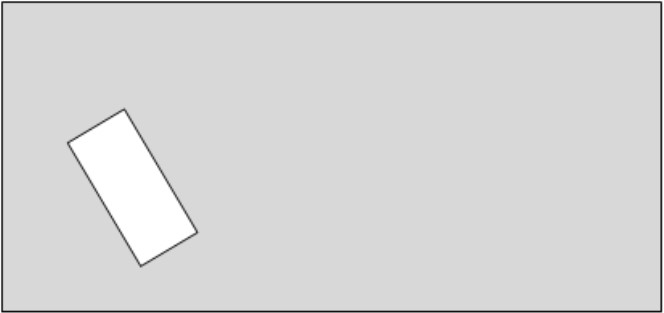
\includegraphics[scale=1]{picture}$$

\begin{center}
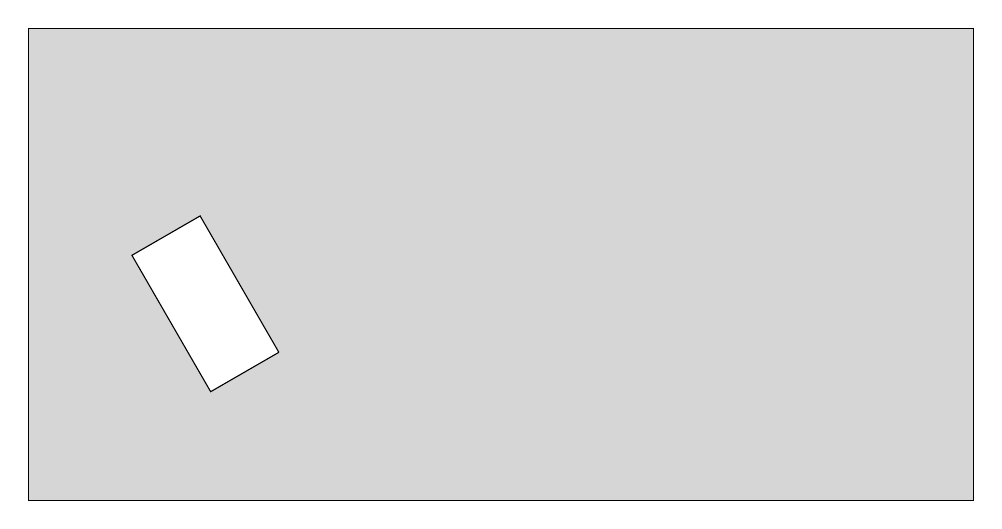
\begin{tikzpicture}
\fill[gray!32!white, draw=black] (0,0) rectangle (12,6);
\fill[white!, draw=black,cm={cos(60) ,-sin(60) ,sin(60) ,cos(60) ,(2.25 cm,2.5 cm)}] (1,0.5) -- (1,-0.5) -- (-1,-0.5) -- (-1,0.5) -- (1,0.5);
\end{tikzpicture}
\end{center}

\begin{solution}
Any straight line through the centre of a rectangle bisects its area (a rectangle is centrally symmetric about its centre). So make the single straight cut pass through \emph{both} centres: the centre of the large rectangle and the centre of the removed rectangular hole.
\newline
That line bisects the large rectangle (it passes through its centre) and also bisects the hole (it passes through the hole's centre). Hence each side of the cut carries (half the large rectangle) $-$ (half the hole) $=$ half the remaining cake. (If the two centres coincide, any line through that common centre works.) 
\end{solution}
% ======================================================

% QUESTION #6

% ======================================================
{\color{white}.}\newline
$\text{\bf {Prerequisites to question 6:}}$ Probability Theory / Calculus.
\section*{\hl{6)}} A random number generator produces independent random variates $x_0,x_1, ...$ drawn uniformly from [0,1], stopping at the first $x_T$ that is strictly less than $x_0$. Prove that the expected value of $T$ is infinite. Suggest, with a brief explanation, a plausible value of $Pr(T\mm{1}=\mm{1}\infty)$ for a real-world (pseudo-) random number generator implemented on a computer.
\begin{solution}
Condition on $x_0=u$. Each later $x_i$ is independently $<u$ with probability $u$, so $T\mid\{x_0=u\}$ is geometric and
$$\mathds{P}(T\ge n\mid x_0=u)=(1-u)^{\,n-1},\qquad \mathds{E}[T\mid x_0=u]=\frac1u.$$
Therefore
$$\mathds{E}[T]=\int_0^1\frac1u\,du=\infty,$$
the divergence coming from $x_0$ near $0$ (it is then very hard to find a smaller value). Equivalently $\mathds{P}(T\ge n)=\int_0^1(1-u)^{n-1}du=\tfrac1n$ and $\sum_n\tfrac1n=\infty$.
\newline
\textbf{Real PRNG.} With exact reals $\mathds{P}(T=\infty)=0$. On a computer the generator emits one of finitely many representable values, say $2^{b}$ of them; if $x_0$ takes the least representable value (in particular if it can equal $0$) nothing is ever strictly smaller, so $T=\infty$. A plausible value is therefore
$$\mathds{P}(T=\infty)\approx2^{-b}\quad(\text{e.g. }2^{-32}\text{ for a }32\text{-bit generator}).$$
\end{solution}
% ======================================================

% QUESTION #7

% ======================================================
{\color{white}.}\newline
$\text{\bf {Prerequisites to question 7:}}$ Elementary Number Theory (quadratic residues).
\section*{\hl{7)}} Prove that there does not exist a four-digit square number $n$ such that $n \equiv 1$ mod 101.
\begin{solution}
Four-digit squares are $m^2$ with $32\le m\le99$ (since $31^2=961$ and $100^2=10000$). If $m^2\equiv1\pmod{101}$ then, as $101$ is prime, $m\equiv\pm1\pmod{101}$, i.e. $m\equiv1$ or $m\equiv100\pmod{101}$. In the range $32\le m\le99$ neither residue occurs ($1$ and $100$ lie just outside it). Hence no four-digit square is $\equiv1\pmod{101}$. 
\end{solution}
% ======================================================

% QUESTION #8

% ======================================================
{\color{white}.}\newline
$\text{\bf {Prerequisites to question 8:}}$ At least one of the following:\newline
{\color{white}.}\hspace{54mm}Ordinary Differential Equations (ODE)\newline
{\color{white}.}\hspace{54mm}Series and integral transforms \newline
{\color{white}.}\hspace{54mm}Partial Differential Equations (PDE)\newline
{\color{white}.}\hspace{54mm}Introduction to Linear Systems\newline
{\color{white}.}\hspace{54mm}Signals and Systems \newline
{\color{white}.}\hspace{54mm}Digital Signal Processing\newline
{\color{white}.}\hspace{54mm}Introduction to communication systems\newline
{\color{white}.}\hspace{54mm}Image Processing\newline
{\color{white}.}\hspace{54mm}Advanced/Algorithms 
\section*{\hl{8)}} The Fourier transform of a function $f(t)$ is defined as:
$$F(\omega) = \bigint_{-\infty}^{+\infty} f(t) e^{-2\pi i \omega t}dt$$
Express the Fourier transform of $f(\alpha t)$ in terms of $F, \alpha$ and $\omega$.
\begin{solution}
This question is very technical and yet it contains profound interpretation of signal processing, we solve by inserting the "scaling" $\alpha$ into the signal and applying the transform:
$$\bigint_{-\infty}^{+\infty} f(\alpha t) e^{-2\pi i \omega t}dt = \frac{1}{\alpha}\bigint_{-\infty}^{+\infty} f(\alpha t) e^{-2\pi i \frac{\omega}{\alpha} \alpha t}d\alpha t = \frac{1}{|\alpha|}F\Big(\frac{\omega}{\alpha}\Big)$$
The absolute value was added because the normalization done by the scaling factor (assuming $\alpha \in \mathds{R}$) has been canceled out with the differential, that the normalization is done only by magnitude. The assumption that $\alpha \in \mathds{R}$ comes from the fact that the question uses Fourier Transform and not Laplace Transform, hence, the attenuation/amplification coefficient is zero.\newnew
This scaling factor compressed or expands the bandwidth, which is the domain length of the frequency to the maximum non-zero harmonics, usually in media it's from the zero frequency, also known as DC current/frequency because the signal is constant in this harmonic, hence there's no oscillation. In communication systems, the carrying frequency is way bigger than the media, and is used to give the media energy to carry throughout the media in the "communication chain".\newnew

\end{solution}
% ======================================================

% QUESTION #9

% ======================================================
{\color{white}.}\newline
$\text{\bf {Prerequisites to question 9:}}$ Data Structures \& Algorithms.
\section*{\hl{9)}} A multiset is a collection of objects, some of which may be repeated. So, for example, $\{ 1, 3, 5, 3, 2, 7, 2\}$ is a multiset. The \textit{multiplicity} of an element in a multiset is the number of times that element occurs in the multiset. Intersections of multisets can be produced in the obvious way: given multisets $A$ and $B$, the multiplicity of an element in $A \cap B$ is the minimum of its multiplicities in each of $A$ and $B$.\vspace{2mm}\newline
Given 2 multisets $A$ and $B$, with unordered elements, outline an algorithm for generating the intersection $A \cap B$.
\begin{solution}
Use a hash map of multiplicities.
\subparagraph*{1.} Scan $A$, building a map $c_A$ with $c_A[x]=$ multiplicity of $x$ in $A$. ($O(|A|)$.)
\subparagraph*{2.} Scan $B$, building $c_B$ likewise. ($O(|B|)$.)
\subparagraph*{3.} For each key $x$ present in (the smaller of) the maps, output $x$ with multiplicity $\min\big(c_A[x],c_B[x]\big)$, treating an absent key as $0$.
\newline
Total time $O(|A|+|B|)$ and space $O(\min(|A|,|B|))$ on average. (Alternatively sort both in $O(n\log n)$ and merge with two pointers, emitting the $\min$ of equal runs.) 
\end{solution}
% ======================================================

% QUESTION #10

% ======================================================
{\color{white}.}\newline
$\text{\bf {Prerequisites to question 10:}}$ Introduction to Computer Science (CS) / Algorithms
\section*{\hl{10)}} Sort the following 16 numbers into 4 sets of 4 and give an explanation for each grouping:\newline
$\{ 1, 2, 3, 4, 4, 5, 5, 8, 9, 11, 13, 17, 25, 32, 49, 128\}$.
\begin{solution}
The two repeats ($4$ and $5$) signal that those numbers belong to two categories each; everything then partitions cleanly:
\subparagraph*{Perfect squares:} $4,\,9,\,25,\,49\ (=2^2,3^2,5^2,7^2)$.
\subparagraph*{Powers of two:} $4,\,8,\,32,\,128\ (=2^2,2^3,2^5,2^7)$.
\subparagraph*{Primes:} $5,\,11,\,13,\,17$.
\subparagraph*{Fibonacci numbers:} $1,\,2,\,3,\,5$.
\newline
The duplicated $4$ is both a square and a power of two; the duplicated $5$ is both a prime and a Fibonacci number -- which is exactly why each appears twice. 
\end{solution}
% ======================================================

% QUESTION #11

% ======================================================
{\color{white}.}\newline
$\text{\bf {Prerequisites to question 11:}}$ Basic number theory / CALC 1
\section*{\hl{11)}} Given 
\[\scaleto{\text{log}_2(11) = 3 + \frac{1}{2 + \frac{1}{5 + \frac{1}{1 + \frac{1}{1 + \frac{1}{1 + \frac{1}{25 + \frac{1}{1 + ...}}}}}}}}{90pt}\]
Which is larger, $2^{128}$ or $11^{37}$?
\begin{solution}
We'll use the logarithmic power rule:
$$\text{log}_a(b^r) = r\mm{1}\text{log}_a(b)\mm{2} \forall b, r\in \mathds{C},\mm{2} a \in \mathds{R}^+$$
On the one hand:
$$\text{log}_2(2^{128}) = 128$$
On the other:
$$\text{log}_2(11^{37}) = 37\mm{1}\text{log}_2(11) = 111 + \textbf{non-negative component}$$
Since 11 isn't any power of 2, it's \textbf{non-negative component} is also irrational, hence the never-ending fraction. Therefore couldn't precisely evaluate the decimal point part (because of infinitely-many digits), we just prove that it's bigger or smaller than: 128-111 = 17. We use the power rule once again, to know the boundaries for our \textbf{non-negative component}:
$$\text{log}_2(8) < \text{log}_2(11) <\text{log}_2(16)$$
$$\text{log}_2(2^3) < \text{log}_2(11) <\text{log}_2(2^4)$$
$$3 < 3 + \textbf{non-negative component} < 4$$
$$0 < \textbf{non-negative component} < 1$$
Each of the never-ending fraction additional component, is positive, hence it's lower bound $\geq 0$. We multiply the \textbf{non-negative component} by 37, and then go over each estimation, and replace the infinitely-many fractional part with zero, thus making it's changing boundary the actual value. Since the fraction is always dividing itself, it's approximating is oscillating between being a lower and upper bound for the actual value, which means that if for 2 times in a row, the estimation is bigger or smaller, we got a case where both a lower and upper bound satisfy the inequality and we can conclude if the value is bigger or smaller respectively.
$$37\cdot(\frac{1}{2 + 0}) = 18.5 > 17$$
Looks "promising", and yet we only began our estimation.
$$37\cdot(\frac{1}{2 + \frac{1}{5 + 0}}) \approx 16.8 < 17$$
The estimation begins to oscillate.
$$37\cdot\Bigg(\frac{1}{2 + \frac{1}{5 + \frac{1}{1 + 0}}}\Bigg) \approx 17.08 > 17$$
$$37\cdot\Bigg(\frac{1}{2 + \frac{1}{5 + \frac{1}{1 + \frac{1}{1 + 0}}}}\Bigg) \approx 16.96 < 17$$
\[\scaleto{37\cdot\Bigg(\mm{2}\frac{1}{2 + \frac{1}{5 + \frac{1}{1 + \frac{1}{1 + \frac{1}{1 + 0}}}}}\mm{2}\Bigg)= 17}{70pt} \]
\[\scaleto{37\cdot\Bigg(\frac{1}{2 + \frac{1}{5 + \frac{1}{1 + \frac{1}{1 + \frac{1}{1 + \frac{1}{25 + 0}}}}}}\Bigg) \approx 16.99 < 17}{90pt}\]
\[\scaleto{37\cdot\Bigg(\frac{1}{2 + \frac{1}{5 + \frac{1}{1 + \frac{1}{1 + \frac{1}{1 + \frac{1}{25 + \frac{1}{1 + 0}}}}}}}\Bigg) \approx 16.99 < 17}{90pt}\]
we got lower and upper boundaries in a row which are both less than 17, hence $2^{128} > 11^{37}$ .
\end{solution} 
{\color{white} .}\newline
Note: Since we're not talking about a singularity point, there will always be a convergence in the approximation. Another reason for the convergence comes from the fact that the approximation of logarithms comes from the approximation of converging geometric series.\newnew
As we all know, time is of the essence in tests, hence it's sufficient to show the 2 boundaries in a row and write those down.\newnew There may be a more difficult/different question, with a different basis and \textbf{NO} approximation given, in that case you should be know how to derive the Taylor series approximation (which is also very handy for general usage), let's give an example with the this question: \newline
\textbf{Q:} Which is larger, $2^{128}$ or $11^{37}$?\newline
\textbf{A:} By simply observing the power on both numbers, we can guess that we're dealing with numbers that are not easy to calculate, and yet they are written in power form, which hints us to apply logarithm with one of their basis (either 2 or 11)
and check if the other is bigger or smaller then the others` power. Since the original question uses log of base 2, we'll use in this case log of base 11:
$$\text{log}_{11}(2^{128}) \lessgtr \text{log}_{11}(11^{37})$$
$$128\mm{1}\text{log}_{11}(2) \lessgtr 37$$
%$$\text{log}_{11}(2) \lessgtr \frac{37}{128}$$
We'll find the approximation of $\text{log}_{11}(2)$ from scratch:\newline
$$\exists \mm{1}x \in \mathds{C} \mm{2}\text{s.t.}\mm{2} |x| < 1$$
(We can also say that $x$ in an element in the disc algebra centered at the origin)
$$f(x) = 1 + x + x^2 + x^3 + ... = \sum_{n = 0}^\infty x^n$$
We want to evaluate the converging sum:
$$1 + x + x^2 + x^3 + ... = 1 + x(1 + x + x^2 + x^3 + ... )$$
Since the series converges, the difference demands to add another element at the end of the series, but because of convergence, the elements go to zero, hence adding or subtracting the last element is like adding or subtracting zero respectively. In case of geometric series which diverges, the sum goes to infinity and then it's like adding or subtracting infinity from the sum, which tells us nothing more than a sum which goes to infinity. 
$$f(x) - xf(x) = 1$$
$$\sum_{n = 0}^\infty x^n = \frac{1}{1 - x}\mm{2}\forall \mm{1}|x| < 1$$
From here we integrate over both sides:
$$\bigint dx \sum_{n = 0}^\infty x^n = \sum_{n = 0}^\infty \bigint dx x^n = \bigint dx \frac{1}{1 - x} \mm{2}\forall \mm{1}|x| < 1$$
$$\text{ln}(1 - x) = -\sum_{n = 1}^\infty \frac{x^n}{n} \mm{2}\forall \mm{1}|x| < 1$$
If it's more convenient to you, it's optional to replace $1 - x \leftrightarrow x$, since it's a specific type of involution (an operation that you apply twice and get the same result, like complex conjugate and transpose) called Legendre transform.
$$\text{ln}(x) = -\sum_{n = 1}^\infty \frac{(1 - x)^n}{n} \mm{2}\forall \mm{1}|1 - x| < 1$$
We want our series to be defined all over the region $x > 0$ in order to plug our values.\newline
By using the logarithmic power rule, we can get back to our logarithm basis: 
$$\frac{\text{ln(x)}}{\text{ln(11)}} = \text{log}_{11}(x)$$
%$$log_{11}(2) = \frac{\sum_{n = 1}^\infty \frac{1}{n}}{\sum_{n = 1}^\infty \frac{(-10)^n}{n}}$$
Now we begin the approximation:
\newline
A caveat first: the series above converges only for $0 < x < 2$, so it reaches $\text{ln}(2)$ -- slowly, and right on the boundary -- but \textbf{not} $\text{ln}(11)$ (for $x = 11$ the terms $\frac{(1 - x)^n}{n} = \frac{(-10)^n}{n}$ blow up). Rather than fight that, we use the near-coincidence $11^2 = 121 \approx 128 = 2^7$ to recast the comparison with arguments close to $1$:
$$\frac{2^{128}}{11^{37}} = \frac{2^2\,(2^7)^{18}}{11\cdot (11^2)^{18}} = \frac{4}{11}\Big(\frac{128}{121}\Big)^{18},$$
so ``$2^{128} \lessgtr 11^{37}$'' is \textit{exactly} the question ``$\big(\frac{128}{121}\big)^{18} \lessgtr \frac{11}{4}$''.
\newline
To converge quickly we upgrade the series: replacing $x \leftrightarrow -x$ in $\text{ln}(1 - x) = -\sum_{n = 1}^\infty \frac{x^n}{n}$ gives $\text{ln}(1 + x) = \sum_{n = 1}^\infty \frac{(-1)^{n - 1} x^n}{n}$, and subtracting the two,
$$\text{ln}\Big(\frac{1 + x}{1 - x}\Big) = 2\Big(x + \frac{x^3}{3} + \frac{x^5}{5} + ...\Big) \mm{2}\forall\mm{1}|x| < 1,$$
which converges geometrically in $x^2$ -- a few terms suffice when $x$ is small.
\newline
$\bullet$\mm{1}\textbf{Numerator} $\text{ln}\frac{128}{121}$: solving $\frac{1 + x}{1 - x} = \frac{128}{121}$ gives $x = \frac{7}{249}$, hence
$$\text{ln}\frac{128}{121} = 2\Big(\frac{7}{249} + \frac{1}{3}\big(\tfrac{7}{249}\big)^3 + ...\Big) = 0.0562397...\mm{2}\Longrightarrow\mm{2} 18\,\text{ln}\frac{128}{121} = 1.012315...$$
$\bullet$\mm{1}\textbf{Denominator} $\text{ln}\frac{11}{4}$: writing $\frac{11}{4} = 2\cdot\frac{11}{8}$, take $\frac{1 + x}{1 - x} = 2$ $(x = \frac{1}{3})$ and $\frac{1 + x}{1 - x} = \frac{11}{8}$ $(x = \frac{3}{19})$:
$$\text{ln}(2) = 2\Big(\tfrac{1}{3} + \tfrac{1}{3\cdot 3^3} + ...\Big) = 0.693147...,\mm{3} \text{ln}\frac{11}{8} = 2\Big(\tfrac{3}{19} + \tfrac{1}{3}\big(\tfrac{3}{19}\big)^3 + ...\Big) = 0.318454...,$$
$$\text{ln}\frac{11}{4} = 0.693147... + 0.318454... = 1.011601...$$
Since $1.012315 > 1.011601$, we have $18\,\text{ln}\frac{128}{121} > \text{ln}\frac{11}{4}$, hence $\big(\frac{128}{121}\big)^{18} > \frac{11}{4}$, and therefore
$$\boxed{2^{128} > 11^{37}}$$
in agreement with the first method.
\newline
The verdict is not delicate once reduced this way: even truncating the (alternating) Mercator series for the numerator after four terms, with $z = \frac{7}{121}$,
$$\text{ln}\frac{128}{121} = \text{ln}(1 + z) > z - \frac{z^2}{2} + \frac{z^3}{3} - \frac{z^4}{4} = 0.0562396...,$$
so $18\,\text{ln}\frac{128}{121} > 1.01231$, while $\text{ln}\frac{11}{4} < 1.01161$; the margin $18\,\text{ln}\frac{128}{121} - \text{ln}\frac{11}{4} \approx 7.1\times 10^{-4}$ far exceeds the truncation error, so the inequality is certain. $\blacksquare$

% ======================================================

% QUESTION #12

% ======================================================
{\color{white}.}\newline
$\text{\bf {Prerequisites to question 12:}}$ Combinatorics
\section*{\hl{12)}} Write $n! = 2^ab$ where $b, n \in \ds{N}$ and $a \in \ds{N} \cup \{ 0 \}$. Prove that $a < n$. 
\begin{solution}
By Legendre's formula the exponent of $2$ in $n!$ is
$$a=\sum_{i\ge1}\Big\lfloor\frac{n}{2^i}\Big\rfloor<\sum_{i\ge1}\frac{n}{2^i}=n\sum_{i\ge1}2^{-i}=n.$$
The inequality is strict: for $2^i>n$ the term $\lfloor n/2^i\rfloor=0$ while $n/2^i>0$. Hence $a<n$. 
\end{solution}
{\color{white}.}\newline
\newpage
\[\scaleto{\bf Long\mm{1}Questions}{20pt}\]
% ======================================================

% QUESTION #1

% ======================================================
{\color{white}.}\newline
$\text{\bf {Prerequisites to question 1:}}$ Stochastic Processes (Markov chains \& random walks).
\section*{\hl{1)}} Alice and Bob play Rock, Paper , Scissors until one or the other is 5 wins ahead. They generate their wins at random, so, in each round, the outcomes are equiprobably win, lose or draw.\newline
After 10 rounds, Alice is 1 ahead. After 13 rounds, one or the other is 1 ahead. At round 20, one of them attains the 5 win lead and the game ends. What is the probability that Alice is the ultimate winner?
\begin{solution}
The lead $L_t$ (Alice's wins minus Bob's) is a lazy random walk: each round $+1,-1,0$ with probability $\tfrac13$ each, absorbed at $\pm5$. We are given $L_{10}=+1$, $|L_{13}|=1$, and that absorption first occurs at round $20$; we want $\mathds{P}(L_{20}=+5)$.
\newline
\textbf{Rounds 10--13 (3 steps from $+1$).} No absorption is possible here, and
$$\mathds{P}(L_{13}=+1\mid L_{10}=1)=\tfrac{7}{27},\qquad \mathds{P}(L_{13}=-1\mid L_{10}=1)=\tfrac{3}{27}.$$
\textbf{Rounds 13--20 (7 steps).} Let $p^{+}(\ell)$, $p^{-}(\ell)$ be the probabilities that, starting at $\ell$, the walk is first absorbed at $+5$, resp. $-5$, exactly at step $7$. A transfer-matrix count (paths staying in $[-4,4]$ for $6$ steps, then stepping out) gives, from $\ell=+1$,
$$p^{+}(1)=\frac{44}{3^{7}},\qquad p^{-}(1)=\frac{6}{3^{7}}.$$
By the reflection $x\mapsto-x$, $p^{+}(-1)=p^{-}(1)$ and $p^{-}(-1)=p^{+}(1)$, so the absorption probability $q=p^{+}+p^{-}=\tfrac{50}{3^7}$ is the same from $+1$ and $-1$.
\newline
Weighting the two starting points by $7$ and $3$,
$$\mathds{P}(L_{20}=+5\mid\text{data})=\frac{7\,p^{+}(1)+3\,p^{+}(-1)}{7q+3q}=\frac{7\cdot44+3\cdot6}{10\cdot50}=\frac{326}{500}=\boxed{\dfrac{163}{250}=0.652}.$$
\end{solution}
% ======================================================

% QUESTION #2

% ======================================================
{\color{white}.}\newline
$\text{\bf {Prerequisites to question 2:}}$ Probability \& Statistics / Randomized Algorithms.
\section*{\hl{2)}} You are monitoring a data stream which is delivering very many 32-bit quantities at a rate of 10 Megabytes per second. You know either:
\subparagraph*{A:} All values occur equally often, $or$ \skipnewline
\subparagraph*{B:} Half of the values occur $2^{10}$ times more often than others (but you dont know anything about which\pnewline{B:} would be the more common values). \newline\newline
You are allowed to read the values off the data stream, but you only have $2^{20}$ bytes of memory.\newline
Describe a method for determining which of the two situations, A or B occurs. Roughly how many data values do you need to read to be confident of your result with a probability of 0.999? [ This is about the 3 sigma level - 3 standard deviations of a normal distribution.]
\begin{solution}
\textbf{Method (collision rate).} The hypotheses differ in their collision probability $c=\sum_v p_v^2$ (the chance that two independent reads are equal):
$$c_A=\frac{1}{2^{32}},\qquad c_B\approx 2^{31}\big(2^{-31}\big)^2=2^{-31}=2c_A$$
(the rare ``light'' values contribute negligibly), so collisions are \emph{twice} as frequent under $B$.
\newline
Memory holds $2^{20}$ bytes $=2^{18}$ thirty-two-bit values, far too few to histogram $2^{32}$ values, so we cannot store every read. Instead fill the table with $s=2^{18}$ reads, then keep reading and count how many later values are \emph{already in the table}. A later read collides with the stored sample with probability $\approx s\,c$ (since $\sum_v p_v\cdot s p_v=s\sum_v p_v^2$), so this hit rate also doubles between $A$ and $B$: about $2^{-14}$ versus $2^{-13}$.
\newline
\textbf{Sample size.} The hit count over $r$ further reads is $\approx$ Poisson with mean $\mu=r\,s\,c$, and $\mu_B=2\mu_A$. Separating means $\mu_A$ and $2\mu_A$ at the $3\sigma$ level needs $\mu_A$ of order a few tens (with $\sigma\approx\sqrt\mu$); taking $\mu_A\approx50$,
$$r\approx\frac{\mu_A}{s\,c_A}=\frac{50}{2^{18}\cdot 2^{-32}}=50\cdot 2^{14}\approx 8\times10^{5},$$
so in total $n\approx 2^{18}+r\sim 10^{6}$ reads. At $10$ MB/s ($\approx2.5\times10^{6}$ values/s) that is well under a second, and it uses only the $2^{20}$ bytes available.
\end{solution}
% ======================================================

% QUESTION #3

% ======================================================
{\color{white}.}\newline
$\text{\bf {Prerequisites to question 3:}}$ Combinatorics / Linear Algebra (transfer matrices \& eigenvalues).
\section*{\hl{3)}} A $2 \times N$ rectangle is to be tiled with $1 \times 1$ and $2 \times 1$ tiles. Prove that the number of possible tilings tends to $kx^N$ as $N$ gets large. Find $x$, to 2 decimal places.
\begin{solution}
Fill the board column by column; the state is which cells of the current column are already covered by a horizontal domino protruding from the left ($\emptyset,\{T\},\{B\},\{T,B\}$). Counting the ways to complete each column (a vertical domino or two monominoes when both cells are free, etc.) gives the transfer matrix
$$M=\begin{pmatrix}2&1&1&1\\1&0&1&0\\1&1&0&0\\1&0&0&0\end{pmatrix},\qquad T_N=(M^{N})_{\emptyset,\emptyset}.$$
(Check: $T_1=2$, $T_2=7$.) Thus $T_N\sim k\,x^{N}$ where $x$ is the largest eigenvalue of $M$. Its characteristic polynomial is
$$\lambda^4-2\lambda^3-4\lambda^2+1=0,$$
whose dominant root is
$$\boxed{\,x\approx3.21\,}\qquad(x=3.2143\ldots).$$
\end{solution}
% ======================================================

% QUESTION #4

% ======================================================
{\color{white}.}\newline
$\text{\bf {Prerequisites to question 4:}}$ Elementary Number Theory.
\section*{\hl{4)}} The Prime Power Divisors (PPD) of a positive integer are the largest prime powers that divide it. For example, the PPD of 450 are 2, 9, 25. Which numbers are equal to the sum of their PPD?
\begin{solution}
Write $m=\prod_i p_i^{a_i}$; its prime-power divisors are the maximal prime powers $p_i^{a_i}$.
\newline
\textbf{Claim: the numbers equal to the sum of their PPD are exactly the prime powers $p^{k}$.}
\newline
If $m=p^{k}$ has one prime, its only PPD is $p^{k}$ and the sum is $p^{k}=m$ -- every prime power qualifies (trivially).
\newline
If $m$ has $r\ge2$ distinct primes, with prime-power parts $X_1,\dots,X_r\ge2$, then ``sum $=$ product'' would need $\prod X_i=\sum X_i$. For $r=2$, $\;X_1X_2-(X_1+X_2)=(X_1-1)(X_2-1)-1\ge(2-1)(3-1)-1=1>0$ (the parts are coprime, so not both $2$), and for $r\ge3$ the product dominates even more. So $\prod X_i>\sum X_i$ strictly, and no such $m$ works.
\newline
Hence the answer is \textbf{precisely the prime powers} $p^{k}\ (k\ge1)$. 
\end{solution}
% ======================================================

% QUESTION #5

% ======================================================
{\color{white}.}\newline
$\text{\bf {Prerequisites to question 5:}}$ Elementary Number Theory (modular arithmetic).
\section*{\hl{5)}} 353, 46, 618, 30, 877, 235, 98, 24, 107, 188, 673 are successive large powers of an integer $x$ modulo a 3-digit prime $p$. Find $x$ and $p$.
\begin{solution}
Successive powers satisfy $a_{k+1}\equiv x\,a_k\pmod p$, hence $a_k^2\equiv a_{k-1}a_{k+1}\pmod p$, so $p\mid(a_k^2-a_{k-1}a_{k+1})$ for every interior $k$. Computing these:
$$a_7^2-a_6a_8=98^2-235\cdot24=3964=2^2\cdot991,\qquad a_8^2-a_7a_9=24^2-98\cdot107=-9910=-2\cdot5\cdot991,$$
and $991$ (a prime) divides all the others too. Hence
$$\boxed{p=991}.$$
Then $x\equiv a_2a_1^{-1}\equiv46\cdot353^{-1}\pmod{991}$. Since $353^{-1}\equiv685\pmod{991}$,
$$x\equiv46\cdot685=31510\equiv\boxed{789}\pmod{991}.$$
(Check: $353\cdot789\equiv46$, $46\cdot789\equiv618$, $618\cdot789\equiv30,\dots$ all hold mod $991$.) 
\end{solution}
% ======================================================

% QUESTION #6

% ======================================================
{\color{white}.}\newline
$\text{\bf {Prerequisites to question 6:}}$ Computational Geometry / Algorithms.
\section*{\hl{6)}} $(X_1, Y_1), (X_2, Y_2), ... (X_n, Y_n)$ are $n$ ordered points in the Cartesian plane that are successive vertices of a non-intersecting closed polygon. \newline\newline
Describe how to find efficiently a diagonal (that is, a line joining 2 vertices) that lies entirely in the interior of the polygon.\newline\newline
Repeated application of this process will completely triangulate the interior of the polygon. Estimate the worst case number of arithmetic operations needed to complete the triangulation.
\begin{solution}
\textbf{Finding an interior diagonal.} Take the lowest vertex (ties broken by leftmost); call it $v$, with polygon-neighbours $u,w$. The interior angle at $v$ is convex. Consider the segment $uw$:
\subparagraph*{$\bullet$} if no other vertex lies inside triangle $uvw$, then $uw$ is an interior diagonal;
\subparagraph*{$\bullet$} otherwise, among the vertices inside $uvw$ pick the one $z$ farthest from the line $uw$; then $vz$ lies entirely inside the polygon and is a diagonal.
\newline
Each search scans all vertices once (a few orientation/area tests apiece): $O(n)$ time.
\newline
\textbf{Triangulating.} A simple $n$-gon needs $n-3$ diagonals and yields $n-2$ triangles. Splitting off one diagonal at a time and recomputing costs $O(n)$ per step over $O(n)$ steps, so the worst case is
$$\boxed{\,\Theta(n^2)\,}\ \text{arithmetic operations.}$$
(Faster methods exist -- $O(n\log n)$ via monotone decomposition -- but the repeated-diagonal method is quadratic.) 
\end{solution}
% ======================================================

% QUESTION #7

% ======================================================
{\color{white}.}\newline
$\text{\bf {Prerequisites to question 7:}}$ Abstract Algebra (groups \& semigroups).
\section*{\hl{7)}} A $semigroup$ is a set $S$ with an associative operation, which we will write as multiplication. That is, $x(yz) = (xy)z$ for all $x,y,z \in S$.
\subparagraph*{a.} Suppose that a finite semigroup $S$ has the property that for all $x$ there is an integer $n > 1$ such that\pnewline{a.} $x^n = x$. Is it true that $S$ is, in fact, a group?
\subparagraph*{b.} Suppose that a finite semigroup $S$ has the property that for all $x$ there is an integer $n > 1$ such that\pnewline{a.} $x^{n+1} = x^n$. Show that the only subsets of $S$ which form a group are of size 1.
\begin{solution}
\textbf{(a) No.} Take the $2$-element \emph{left-zero} semigroup $S=\{a,b\}$ with $xy=x$ for all $x,y$. Then $x^2=x$, so $x^n=x$ with $n=2>1$ for every $x$; but $S$ has no identity (an $e$ would need $ey=y$, while $ey=e$), so it is not a group. (Any non-trivial semilattice, e.g. $\{0,1\}$ under multiplication, is another counterexample.)
\newline
\textbf{(b)} For each $x$ the powers $x,x^2,\dots$ stabilise: once $x^{n+1}=x^{n}$ they stay constant and $x^{n}$ is idempotent. Suppose $G\subseteq S$ forms a group with identity $e$. For $g\in G$ all powers $g^m$ lie in $G$, and $g^{n+1}=g^{n}$ holds in $S$; cancelling in the group gives $g=e$. So every element of $G$ equals $e$, i.e. $|G|=1$. 
\end{solution}
% ======================================================

% QUESTION #8

% ======================================================
{\color{white}.}\newline
$\text{\bf {Prerequisites to question 8:}}$ Theory of Computation (automata \& formal languages).
\section*{\hl{8)}} A \textit{finite state machine M} consists of a finite set of states, each having two arrows leading out of it, labelled 0 and 1. Each arrow from state $x$ may lead to any state (both may lead to the same state, which might be $x$).\newline\newline
One state is labelled the "initial" state; one or more states are labelled "accept". The machine reads a finite binary string by starting at "initial" and considering each symbol in the string in turn, moving along the arrow with that label to the next state until the end of the string is reached. If the final state is labelled "accept", the machine $accepts$ the string.\newline\newline
The \textit{language, L(M)} of the machine is the set of all the finite binary strings that the machine accepts.
\subparagraph*{a.} Design a machine whose language is all palindromic strings of length 6 (\textit{i.e.}, strings for which the last \pnewline{a.}3 symbols are a reflection of the first 3).
\subparagraph*{b.} Suppose that \textit{L(M)} is not finite. Show that the number of strings in \textit{L(M)} of length $n$ or less grows \pnewline{b.}linearly with $n$.
\subparagraph*{c.} Show that there is no machine such that \textit{L(M)} consists of all twice-repeated strings.
\begin{solution}
\textbf{(a)} Length is bounded by $6$, so the language is finite, hence regular. Build a depth-$3$ binary trie recording the first three bits $s_1s_2s_3$ ($1+2+4+8$ states). From each of the $8$ leaves, reading $s_4,s_5,s_6$ must reproduce $s_3,s_2,s_1$: each correct bit advances toward a unique \textbf{accept} state, any wrong bit (or a $7$th symbol) goes to a single non-accepting \textbf{dead} state. This accepts exactly the length-$6$ palindromes.
\newline
\textbf{(b)} Let $M$ have $k$ states. If $L(M)$ is infinite, some accepting path repeats a state, i.e. contains a cycle of length $\ell$ with $1\le\ell\le k$. Pumping that cycle $j=0,1,2,\dots$ times yields accepted strings of lengths $L_0+j\ell$. Hence the number of accepted strings of length $\le n$ is at least $\big\lfloor(n-L_0)/\ell\big\rfloor+1\ge(n-L_0)/k$ -- i.e. it grows at least linearly in $n$.
\newline
\textbf{(c)} Suppose some $M$ accepted exactly $\{ww:w\in\{0,1\}^\ast\}$, with pumping length $k$. Take $s=0^{k}1\,0^{k}1=ww$ with $w=0^k1$. Pumping forces $s=xyz$ with $|xy|\le k$, so $y=0^{j}$ ($j\ge1$) and $xy^2z=0^{k+j}1\,0^{k}1$, which is \emph{not} of the form $ww$ (a string $0^{a}1\,0^{b}1$ is a square only if $a=b$). Contradiction, so no such machine exists. 
\end{solution}
% ======================================================

% QUESTION #9

% ======================================================
{\color{white}.}\newline
$\text{\bf {Prerequisites to question 9:}}$ Algorithms (dynamic programming).
\section*{\hl{9)}} Suppose $P$ is a permutation on $\{ 0, 1, ... , n - 1\}$. We want to know the length of the longest monotonically increasing subsequence. That is, the largest $m$ such that there exist monotonically increasing $j_1, j_2, ... , j_m$ for which $P(j_1), P(j_2), ... , P(j_m)$ are also monotonically increasing.\newline\newline
Describe an algorithm that will determine $m$ using $O(n^2)$ time and $O(n)$ memory.
\begin{solution}
Dynamic programming. For each index $i$ let
$$L[i]=1+\max\{\,L[j]:j<i,\ P(j)<P(i)\,\}\qquad(\text{and }L[i]=1\text{ if no such }j).$$
Then the answer is $m=\max_i L[i]$, the length of the longest increasing subsequence (each $L[i]$ is the best such subsequence ending at $i$).
\newline
Computing $L[i]$ scans all $j<i$, so the total time is $O(n^2)$; only the array $L$ (and $P$) is stored, giving $O(n)$ memory. (Patience sorting attains $O(n\log n)$, but the DP already meets the requested bounds.) 
\end{solution}
% ======================================================

% QUESTION #10

% ======================================================
{\color{white}.}\newline
$\text{\bf {Prerequisites to question 10:}}$ Combinatorics (pigeonhole principle).
\section*{\hl{10)}} Given 541 points in the interior of a circle of unit radius, show that there must be a subset of 10 points whose diameter (the maximum distance between any pair of points) is less than $\sqrt{2}/4$.
\begin{solution}
Cover the unit disk with the axis-aligned grid of squares of side $\tfrac14$. Such a square has diameter $\tfrac{\sqrt2}{4}$; using \emph{half-open} squares (top/right edges excluded) gives a genuine partition in which any finite set of points has diameter \emph{strictly} less than $\tfrac{\sqrt2}{4}$.
\newline
Only squares meeting the disk matter. A square in one quadrant with near corner $(i/4,j/4)$ meets the disk iff $i^2+j^2<16$; counting gives $15$ per quadrant, so $4\times15=60$ squares in all. With $541=60\cdot9+1$ points in $60$ cells, pigeonhole forces some cell to contain at least
$$\Big\lceil\tfrac{541}{60}\Big\rceil=10$$
points. Those $10$ points lie in one $\tfrac14$-square, so their pairwise distances -- and hence their diameter -- are $<\tfrac{\sqrt2}{4}$. 
\end{solution}
% ======================================================

% QUESTION #11

% ======================================================
{\color{white}.}\newline
$\text{\bf {Prerequisites to question 11:}}$ Combinatorics / Graph Theory (double counting).
\section*{\hl{11)}} Show how the edges of a cube (8 vertices; 12 edges) can be directed so that some vertices have all edges  pointing out (\textit{i.e.} directed away from the vertex), and the remainder have one edge out and two in.\newline\newline
Suppose the edges of a 5-dimensional hypercube (32 vertices, 80 edges) are directed so that all vertices have either 5 edges pointing out, or 4 edges in and 1 out. Show that every 4-dimensional subcube must contain precisely 6 of the 5-out vertices.
\begin{solution}
\textbf{Cube.} If $s$ vertices are ``all-out'' (out-degree $3$) and the rest have out-degree $1$, summing out-degrees gives $3s+(8-s)=12$, so $s=2$. Construction on $\{0,1\}^3$: make $000$ and $111$ the two sources (orient their three edges outward). The remaining six edges join $\{100,010,001\}$ to $\{110,101,011\}$ in a $6$-cycle
$$100\!-\!110\!-\!010\!-\!011\!-\!001\!-\!101\!-\!100;$$
orient this cycle consistently. Then each of the other six vertices has out-degree $1$ (its cycle edge) and in-degree $2$ (one from a source, one from the cycle). $\blacksquare$
\newline
\textbf{$5$-cube.} Out-degrees give $5s+(32-s)=80$, so there are exactly $s=12$ ``$5$-out'' vertices. Fix a $4$-dimensional subcube (facet) $F$ -- there are $5\cdot2=10$ of them. $F$ is a $4$-cube with $16$ vertices and $32$ internal edges. A vertex's internal out-degree is $4$ if it is a source and $0$ or $1$ otherwise; summing to the $32$ internal edges,
$$4a_F+b_F=32,\qquad 0\le b_F\le16-a_F,$$
where $a_F$ counts the sources in $F$. This forces $16\le3a_F$, i.e. $a_F\ge6$. Finally each source lies in exactly $5$ facets, so over the $10$ facets $\sum_F a_F=5\cdot12=60$, an average of $6$. Since every $a_F\ge6$ and they average $6$, every facet has exactly
$$\boxed{a_F=6}$$
of the $5$-out vertices. 
\end{solution}
\newpage
% ======================================================

% 						TEST #3

% ======================================================

\begin{center}
\Large
\bf Proposed solution to "Sample GCHQ Mathematics Applications Test"\\
\vspace{2mm} Test $\#$3
\end{center}
% ======================================================

% QUESTION #1

% ======================================================
{\color{white}.}\newline
$\text{\bf {Prerequisites to question 1:}}$ Introduction to Cryptography.
\section*{\hl{1)}} A hash is a one-way (hard to invert) function $H$ which can take an input of any size and produce a fixed-size output. Typical requirement for good hash functions are:
\subparagraph*{$\bullet$} Pre-image resistance: given $H(A)$, it is very difficult to find $A$.\skipnewline
\subparagraph*{$\bullet$} Second pre-image resistance: given $A$, it is very difficult to find $B \neq A$ such that $H(A) = H(B)$.\skipnewline
\subparagraph*{$\bullet$} Collision-resistance: it is very difficult to find $A,B,$ with $A \neq B$, such that $H(A) = H(B)$.\newline\newline
Alice wishes to vote in an upcoming election for which there are just two voting options. She can securely share a verification value with the voting authority in advance but will be voting over an untrustworthy channel.\newline\newline
Consider the following voting scheme based on a hash function $H$.
\subparagraph*{$\bullet$} Alice chooses two secret keys, $s_1$ and $s_2$.\skipnewline
\subparagraph*{$\bullet$} Alice generates the verification value $H(H(s_1)||H(s_2))$. This value is shared with the voting authority \pnewline{$\bullet$}in advance of the election.\skipnewline
\subparagraph*{$\bullet$} If Alice wishes to vote 'yes' she sends $\big(s_1, H(s_2)\big)$; if she wishes to vote 'no' she sends 
$\big(H(s_1), s_2\big)$.\newline\newline
Note that the symbol $||$ is used to denote the concatenation of two values.
\subparagraph*{a.} i) How does the authority determine how Alice voted? \pnewline{a.}
ii) Why are the secret keys used in this voting scheme one-time use only? \pnewline{a.}
iii) Justify why an adversary cannot change Alice's vote. 
\subparagraph*{b.} Without increasing the number of secret keys nor increasing the size of the verification value, how can \pnewline{b.}you generalise this scheme to voting for one of 8 options? Justify why an adversary still cannot change \pnewline{b.}Alice's vote in your proposed scheme.
\subparagraph*{c.} Discuss whether the property of the second pre-image resistance is required in the choice of $H$ for this \pnewline{c.}voting scheme. 
\begin{solution}
\textbf{a. i)} The authority holds $V=H\big(H(s_1)\Vert H(s_2)\big)$. For a ``yes'' it receives $\big(s_1,H(s_2)\big)$ and checks $H\big(H(s_1)\Vert H(s_2)\big)=V$ (hashing the first component once); for a ``no'' it receives $\big(H(s_1),s_2\big)$ and checks $H\big(H(s_1)\Vert H(s_2)\big)=V$ (hashing the second component once). Exactly one interpretation reproduces $V$, revealing the vote.
\newline
\textbf{ii)} A vote reveals one pre-image (say $s_1$) over the open channel, so it is no longer secret; reusing the same $V$ would let anyone who saw it replay or forge with the now-public key. Hence one-time use.
\newline
\textbf{iii)} To flip a ``yes'' $(s_1,H(s_2))$ into a ``no'' the adversary needs $s_2$, but only has $H(s_2)$ -- recovering $s_2$ is a pre-image computation (infeasible). Any other accepted pair needs a pre-image of $V$ (or a collision). So the vote cannot be changed.
\newline
\textbf{b. (8 options).} Use two hash chains of length $7$: commit to $V=H\big(H^{7}(s_1)\Vert H^{7}(s_2)\big)$ (same size, still two secrets). To vote $k\in\{0,\dots,7\}$ send $\big(H^{k}(s_1),H^{7-k}(s_2)\big)$; the authority applies $H^{7-k}$ and $H^{k}$ and checks $V$. An adversary can only hash \emph{forward}, so changing $k$ would need to go backward on one chain (a pre-image) -- infeasible. This gives $8$ options with no extra keys and no larger commitment.
\newline
\textbf{c.} Second pre-image resistance is \emph{not} required. The attacker's only useful inversion is recovering an unrevealed secret (a pre-image) or a pre-image of $V$; a second pre-image (a different input with the same hash, starting from a \emph{known} input) does not help change the vote. Pre-image resistance is the property relied on; collision resistance is irrelevant here since Alice forms her own honest commitment. 
\end{solution}\newpage
% ======================================================

% QUESTION #2

% ======================================================
{\color{white}.}\newline
$\text{\bf {Prerequisites to question 2:}}$ Cryptography \& Network Security.
\section*{\hl{2)}} Alice and Bob are good friends who lead busy lives and rarely get a chance to catch up in person. They wish to communicate over an insecure channel by securing their messages using a symmetric encryption algorithm. Eve intends to cause as much disruption as possible to communicate between Alive and Bob, and in particular wishes to read the messages sent. \newline\newline
To start communications in an encrypted manner Alive sends Bob an unencrypted message over the channel. The message contains instructions on how they can encrypt their messages as follows:
\subparagraph*{-} Generate a key, $K_1$, by cryptographically hashing the date. \skipnewline
\subparagraph*{-} Use this key to encrypt a message before sending, or decrypt any messages received that day.
\subparagraph*{a.} Explain any problems with this system. How may Eve read any encrypted messages?\newline\newline
Alice realises the error she made. She randomly creates a new symmetric key, $K_2$, for communications and meets with Bob to exchange the key. Both subsequently store the key on their devices which connect to the insecure channel. 
\subparagraph*{b.} Eve sees messages being exchanged between Alice and Bob. What can she do without knowledge of the \skipnewline\pnewline{b.}new key, $K_2$? How could Eve obtain the new key?\newline\newline
Alice receives the same messages from Bob multiple times. She suspects Eve is repeatedly sending an old message from Bob. She devises a replay protection mechanism. Within each encrypted message Alice and Bob send they include the time. When a message is received, the time is checked and if it falls within the last 30 seconds they trust the message is new.
\subparagraph*{c.} What problems may occur in this new scheme? How may Eve disrupt things further? Suggest an \pnewline{c.} improvement to this scheme, and explain how it mitigates these flaws. \newline\newline
Alice suspects that Eve may have discovered the encryption key, $K_2$. She is getting fed up of having to meet with Bob to exchange keys, and researches Public Key Cryptography.\newline\newline
During one of their infrequent meetings, Alice explains to Bob how they can use the RSA cryptography system to communicate securely. Alice generates integers $N , e$ and $d$ such that for any integer $M$, we have 
$$M^{ed} \equiv M\mm{1} \text{mod}\mm{1} N$$
She publishes $N$ and $e$, but keeps $d$ private. If someone wishes to send a message to Alice, they compute and send $Z \equiv M^e \mm{1} \text{mod} \mm{1} N$. Alice can recover $M$ by computing $M \equiv Z^d \mm{1} \text{mod} \mm{1} N$.
\subparagraph*{d.} How can Alice prove Bob that a message could only have been written by her? This process is known\pnewline{d.} as signing the message.\newline\newline
Alive gives Bob her public key, $N$ and $e$, on a USB flash drive. Unfortunately, Bob loses the flash drive on the train. 
\subparagraph*{e.} Does Alice need to generate a new key pair? Justify your answer.
After hearing of Bob's carelessness, Alice sends her public key to Bob in an unencrypted email.
\subparagraph*{f.} Explain how Eve, with the ability to intercept and modify messages, could eavesdrop on their \pnewline{f.} conversations without either of them knowing. Why would this not be a problem if Bob hadn't lost the \pnewline{f.} flash drive? \newline\newline
Alice is pleased with her secure instant messaging system. She decides to develop it further and releases Alice Messenger System (AMS) to the other residents of her town. Word travels fast, and soon all the townfolk are aware of Alice's system, and know her public key. \newline\newline
Alice's friend Charlie wants to use AMS. He generates a key pair and hands Alice his public key on a USB flash drive he found on the train. Alice signs the message "Charlie's public key is: [Public Key]". This message, along with its signature, is called a certificate, which she gives to Charlie.
\subparagraph*{g.} Given that everyone trusts Alice, how can Charlie use his certificate to convince any resident that a \pnewline{g.} message was written by him? \newline
Alice would like to sign certificates for everyone in the town. She announces to everyone that she would like them to email her with their name and public key, and she will respond with a certificate.
\subparagraph*{h.} Comment on the suitability of this method of certification. Suggest any faults and improvements. \newline
Alice designed AMS so that when a character is typed, it is interpreted as an integer between 0 and 255, then RSA encrypted and sent to the recipient where it is immediately decrypted and displayed on their screen. 
\subparagraph*{i.} Suggest any faults and improvements for this scheme. How does this implementation affect an attacker's \skipnewline\pnewline{i.}ability to recover a private key? 
\begin{solution}
\textbf{a.} The date is public and low-entropy, and the scheme is sent in the clear, so Eve computes $K_1=H(\text{date})$ herself and decrypts everything. (Never derive keys from public/predictable data.)
\newline
\textbf{b.} Without $K_2$ Eve cannot read the traffic, but she can still do traffic analysis (timing, lengths, frequency), block/delay/reorder/replay, and tamper (corrupting ciphertext -- undetectably if there is no integrity check). She could obtain $K_2$ by compromising an endpoint (the key is stored on Internet-connected devices: malware, theft), side channels, or weak-cipher cryptanalysis.
\newline
\textbf{c.} A $30$-second window still lets Eve replay within it, and it requires synchronised clocks (drift causes false rejects/accepts); if timestamps are not integrity-protected she can alter them. Better: attach a unique nonce / monotonic sequence number to each message plus a MAC (use authenticated encryption); the receiver rejects duplicates and out-of-order messages. This stops replay regardless of timing and detects tampering, without relying on clocks.
\newline
\textbf{d.} Alice \emph{signs}: she sends $S=H(M)^{d}\bmod N$ with $M$; anyone verifies $S^{e}\equiv H(M)\pmod N$ using her public $(N,e)$. Only the holder of $d$ could produce $S$, proving authorship and integrity.
\newline
\textbf{e.} No. Only the \emph{public} key was lost; it is meant to be public and does not expose $d$. Alice simply re-sends it (authentically). A new pair is needed only if the \emph{private} key leaks.
\newline
\textbf{f.} Sending the public key over unauthenticated email enables a man-in-the-middle: Eve replaces Alice's key with her own, so Bob encrypts to Eve, who decrypts, reads/alters, and re-encrypts to Alice -- invisibly. The USB drive was an \emph{authenticated} out-of-band channel, so had Bob kept it he would hold Alice's genuine key and the substitution would fail. (For public keys, authenticity -- not secrecy -- is what matters.)
\newline
\textbf{g.} Charlie shows the certificate ``Charlie's public key is [PK]'' together with Alice's signature on it. Any resident verifies that signature with Alice's trusted key, thereby trusting that PK is Charlie's; Charlie then signs his messages and residents verify with the certified PK. (Alice acts as a certificate authority.)
\newline
\textbf{h.} Certifying from emailed name$+$key is unsafe: Alice cannot tell that the sender really owns that name/key, so Eve can have ``Dave's key'' certified as \emph{her} key and impersonate Dave. Improvements: verify identity out-of-band (in person / ID) and require proof-of-possession of the private key (sign a challenge) before issuing a certificate.
\newline
\textbf{i.} Encrypting one character (a value $0$--$255$) with deterministic textbook RSA is fatal: an attacker encrypts all $256$ possibilities under the public key and matches -- a dictionary attack that decrypts everything \emph{without} the private key -- and equal characters give equal ciphertexts (frequency analysis). It does not materially ease recovery of $d$ (that still needs factoring $N$), but confidentiality is already lost. Fix: hybrid encryption (RSA-wrap a random symmetric key, then AES) with randomised padding (OAEP) and authenticated encryption -- never per-character textbook RSA. 
\end{solution}\newpage
% ======================================================

% QUESTION #3

% ======================================================
{\color{white}.}\newline
$\text{\bf {Prerequisites to question 3:}}$ At least one of the following:\newline
{\color{white}.}\hspace{54mm}Information theory\newline
{\color{white}.}\hspace{54mm}Advanced random signals and noise\newline
{\color{white}.}\hspace{54mm}Advanced Stat Mech / Thermodynamics\newline
\section*{\hl{3)}} \textbf{Shannon Entropy} is a measure of randomness of a discrete random variable X hich can be defined as
$$H(X) = -\sum^{n}_{i = 0}P(x_i)\text{log}(P(x_i))$$
where each $x_i$ is a possible value of $X$.\newline\newline
For the purposes of cryptographic investigation we consider $X$ to be the output of a random number generator, with $x_i$ denoting all the possible values it could take. By using logarithms in base 2, we can think of entropy in terms of bits. Some key properties of entropy include:
\subparagraph*{$\bullet$} Data can have less entropy than the total number of bits, but not more.
\subparagraph*{$\bullet$} Different length blocks of data can contain the same amount of entropy.
\subparagraph*{$\bullet$} Identical length blocks of data can contain different amounts of entropy.\newline\newline
This is a very important concept in cryptography, particularly when considering cryptographic keys and passwords. For instance, an 8 byte key, where the value of each byte is independent and uniformly distributed, can have up to 64 bits of entropy. We can see this by applying the above formula to each byte to obtain 
$$-\sum_{i = 0}^{255}P(i)\cdot\text{log}\big( P(i) \big) = -256 \cdot (\frac{1}{256}\cdot \text{log}_22^{-8}) = 8,$$
and then summing this over all the bytes. \newnew
However, it those bytes can only take the values 1 or 0, then we see that the entropy in the key cannot exceed 8 bits, since $\big(-(\frac{1}{2}\cdot \text{log}_22^{-1}+\frac{1}{2}\cdot \text{log}_22^{-1}) + 0 + 0 + ...\big) = 1$
\subparagraph*{a.} (i) If each byte in this 64 bit key has exactly 1 non-zero bit, and this bit can take any position in the \pnewline{a.}{\color{white}(i) }byte with equal probability, how much entropy is there in the entire key?
\pnewline{a}(ii) The entropy in a stream is preserved under 1-to-1 map. State a 1-to-1 map from the 64 bit space \pnewline{{a.}(ii)} in (i) such that the resultant stream will have maximal entropy.\newnew
If we take 2 independent streams $A$ and $B$ of 64 bits and concatenate them, then $A||B$ has the sum of the entropy in $A$ and $B$.
\subparagraph*{b.} (i) If $A$ and $B$ are dependent, in that $B = F(A)$, where $F$ is an 1-to-1 map, how much entropy does \pnewline{b.}{\color{white}(i) }$A||B$ have?\newpage
\subparagraph*{\color{white} b}(ii) If $F$ is not invertible (say a cryptographic hash) how would that affect your answer? Justify your \pnewline{b.}{\color{white}(ii)}reasoning briefly.\newnew
In a cryptographic system, in order for a key to have full entropy, random data is taken from a random source and pooled into a much larger store than the size of the key to be generated. When a key is required, the large quantity of data is processed and compacted to produce the key using a non invertible function. This ensures that if there is relatively little entropy in the collected data, the resultant key will have higher entropy.\newnew
Consider the following example system. We have a timer which starts at zero, and has accuracy to 1 microsecond ($10^{-6} $ seconds). We have a perfect random source which will reset the timer to 0 at most 1 second after the previous reset. The value of the timer at reset is read off as a 64 bit value and added to our entropy pool. When a 64 bit key is needed, all the 64 bit timer values in the entropy pool are bitwise XORed.\newnew
Bitwise XORing 2 data streams will result in a stream with greater than or equal entropy to both the input streams.
\subparagraph*{c.\color{white} .} i) How much entropy is in each 64 bit timer value (use the fact that $2^{10} \approx 1000$ to help with your \pnewline{{c.\color{white}} i)}estimate).
\subparagraph*{\color{white} b.}ii) How many of these values (assuming independence) would need to be concatenated to produce a \pnewline{{c.\color{white}..}i)}value with $\geq 64 $ bits of entropy.
\subparagraph*{\color{white} b}iii) What is wrong with the suggested XOR combining function? Suggest a better function to produce \pnewline{{c.\color{white}..}i)}a high entropy 64 bit output.
\begin{solution}
\textbf{a. i)} Each byte has $8$ equally likely states (the position of its single $1$), i.e. $\log_2 8=3$ bits; the $8$ independent bytes give $8\times3=\boxed{24}$ bits.
\newline
\textbf{ii)} Map each byte to the $3$-bit index of its non-zero bit and concatenate the eight indices. This $1$-to-$1$ map sends the key to a uniform $24$-bit string, which has the maximal $24$ bits of entropy for its length.
\newline
\textbf{b. i)} Since $B=F(A)$ with $F$ invertible, $A$ and $B$ determine each other, so $H(A\Vert B)=H(A)$ (no extra entropy) -- at most $64$ bits, not $128$.
\newline
\textbf{ii)} If $F$ is non-invertible (a hash), the \emph{joint} entropy is unchanged: $H(A\Vert B)=H(A)+H(B\mid A)=H(A)$, because $B$ is still a deterministic function of $A$. (Only $H(B)$ drops below $H(A)$.)
\newline
\textbf{c. i)} The reset time is uniform over up to $1\text{ s}/1\,\mu\text{s}=10^{6}$ ticks, so each timer value carries $\log_2 10^{6}\approx\log_2 2^{20}=\boxed{20}$ bits (using $2^{10}\approx10^3$).
\newline
\textbf{ii)} Entropy adds under concatenation, so $\lceil 64/20\rceil=\boxed{4}$ values are needed for $\ge64$ bits.
\newline
\textbf{iii)} XOR is wrong because all the entropy sits in the low $\sim\!20$ bits (the values are $<2^{20}$, so the top $\sim\!44$ bits are always $0$); XORing such values leaves those high bits zero, so the result keeps only $\sim\!20$ bits, never $64$. Instead pool $\ge4$ samples and run them through a non-invertible cryptographic hash truncated to $64$ bits, which diffuses the entropy across all output bits. 
\end{solution}\newpage
% ======================================================

% QUESTION #4

% ======================================================
{\color{white}.}\newline
$\text{\bf {Prerequisites to question 4:}}$ Computer \& Network Security.
\section*{\hl{4)}} SecretStore is an online cloud computing service which is designed to allow users to store their files, encrypted, on its servers, without the server administrators being able to decrypt them. \newnew
To set up SecretStore, the user must provide a username and password for their choice on the login page. The SecretStore software computes a hash of their passwords, then sends the results and the username to the SecretStore server which saves them. When the user needs to prove who they are to the server, they only send this hash; this way, SecretStore never needs to know their actual password.\newnew
If a user supplies the wrong password, the server sends a message back telling the user they have entered the incorrect password. The SecretStore software keeps track of how many times this has happened that day in a file stored on the user's computer; once a person has failed to log in three times, it refuses to send further attempts to the server until the next day (at which point it deletes the log file).
\subparagraph*{a.} How might an attacker gain access to one of the users` accounts, if they can get to the login page but \pnewline{a.}have no direct access to the sever, any users` machine or the communications between the two?\skipnewline
\subparagraph*{b.} What measures could SecretStore employ to protect against such attempts?\newnew
Once a user has logged in, she can download any of her encrypted files. The SecretStore software on her computer uses the hash of her password as a key to encrypt or decrypt files. This way, the server never sees the unencrypted files, and they are never sent over the internet.
\subparagraph*{c.} How could an attacker gain or deny access to or modify the user`s files if:\newline
\pnewline*{\color{white} c..} i) He is able to intercept messages between the user and the server?
\pnewline*{\color{white} c.} ii) He had access to the user`s computer?
\subparagraph*{d.} What measures might the user or the server employ to prevent or mitigate against these attacks? \newnew
To let users share files with each other SecretStore decide to implement a new system using public key cryptography. When setting up SecretStore, each user generates a public and a private key. Anyone can encrypt a file with the public key, but only the person who knows the private key can then decrypt it.\newnew
To share files with others, one user generates a secret File Key (FK) by hashing the number of milliseconds since midnight. The user then encrypts a copy of the FK with each sharer's public key, and sends the results to the server. When one sharer wants to view or upload a file, they download the version of the FK which was encrypted with their public key, decrypt it using their private key, then use that to encrypt or decrypt the files themselves. The FK replaces the password hash for encrypting these files. 
\subparagraph*{e.} Suggest a weakness in the encryption used in the sharing group which might allow an attacker to decrypt\pnewline{a.}an encrypted file. How might you improve the system to remove this weakness? 
\subparagraph*{f.} If an attacker had the ability to interfere with the set-up of the sharing group, could he use this capability \skipnewline\pnewline{f.}to ensure that he could later read the files which the users encrypt?
\subparagraph*{f.} Are there any further measures SecretStore could take to improve their security?
\begin{solution}
\textbf{a.} The three-strike limit is enforced \emph{on the client}, so an attacker using their own client (or calling the server directly) ignores it and brute-forces / dictionary-attacks passwords against the un-throttled server.
\newline
\textbf{b.} Enforce rate-limiting and lockout \emph{server-side} (per account); store passwords with a slow, \emph{salted} hash (bcrypt/scrypt/Argon2); add multi-factor authentication and monitoring.
\newline
\textbf{c. i)} If the channel is unencrypted, the password \emph{hash} -- which is both the auth token \emph{and} the file-encryption key -- is captured: the attacker can impersonate the user \emph{and} decrypt her files, or simply corrupt transfers (denial of service).
\newline
\textbf{ii)} With access to her machine the attacker reads the stored hash (= credential and key), keylogs the password, or reads decrypted files -- full compromise.
\newline
\textbf{d.} Always use TLS; do not reuse the password hash as both token and key (derive separate keys); use challenge--response authentication so the static hash cannot be replayed. Against endpoint compromise: full-disk encryption, no persisted key, MFA, session timeouts.
\newline
\textbf{e.} The File Key is $H(\text{ms since midnight})$, with only $\sim\!2^{27}$ ($<10^{8}$) possibilities and predictable from the creation time -- brute-forceable. Generate the FK from a cryptographically secure RNG (a full $128$/$256$-bit random key).
\newline
\textbf{f.} Yes: by interfering with setup the attacker injects \emph{his own} public key as a ``sharer'', so the FK is also encrypted to him and he can read every file. Prevent this by authenticating the sharers' public keys (certificates / verified identities).
\newline
\textbf{g.} Further: authenticated public keys, authenticated encryption of files (integrity), per-file random keys, key rotation, server-side throttling with salted slow hashing, MFA, signed client software, and audit logging. 
\end{solution}\newpage
% ======================================================

% QUESTION #5

% ======================================================
{\color{white}.}\newline
$\text{\bf {Prerequisites to question 5:}}$ Mathematical Statistics / Detection \& Estimation Theory.
\section*{\hl{5)}} Suppose you are trying to detect illicit activity on a system. You are able to observe vast amounts of data - more than you could possibly store and process offline. For simplicity, assume that the data come from some uninvariant process, and that illicit behavior is represented as a sudden and persistent (at least in the short-term) change in this process. You are responsible for developing analytics / statistical tests to identify such changes.
\subparagraph*{a.} Suggest what properties these analytics need to have to be of practical use. \newnew
One commonly used changepoint detection test is the CUSUM algorithm. It performs optimally when the pre-change mean and variance of the process are known, $\mu_1$ and $\sigma_1$ is required. Then the statistics $S_j$ is defined as:
$$S_0 = \mu_1$$
$$S_0 = \text{max}0, S_{j-1} + x_j - k\mu_1,$$
where $x_j$ is the $j^{th}$ observation of the process, $k$ is a control parameter, tuned depending on the magnitude of the change one is trying to detect. If $S_j$ exceeds some threshold $h\sigma_1$ (where $h$ is another control parameter), then a change is declared.
\subparagraph*{b.} In a streaming environment, where we only store the most recent few observations and the udnerlying \pnewline{b.}process may drift over time, suggest reasons why the CUSUM algorithm as described above may not \pnewline{b.}be suitable. \newnew
The most recent observations in a data stream tend to give us the most accurate view of the current behavior. So, we want to use adaptive estimation techniques. Consider a set of $N$ observations, $x_1, x_2, ... , x_N$. Recall that the usual arithmetic mean is given by 
$$\bar{x}_N = \frac{1}{N}\sum_{k = 1}^N x_k.$$
Adaptive estimation introduces an exponential $forgetting factor, \mm{1}\lambda \in [0,1].$ The \textbf{forgetting factor mean} is defined as: 
$$\bar{x}_{N,\lambda} = \frac{1}{w_{N,\lambda}}\sum_{k = 1}^N \lambda^{N-k}x_k,$$
where $w_{N,\lambda} = \sum_{k = 1}^N \lambda^{N-k}$.
\subparagraph*{c.} Describe how $\bar{x}_{\lambda}$ behaves for each of the 3 cases $\lambda = 0 , \lambda = 1, 0 < \lambda < 1$.
\subparagraph*{d.} i) Assume that $x_1, x_2, ... , x_N$ are sampled from random variables $X_1, X_2, ... , X_N$ all of which have \pnewline{d..i)}}expected value $\mu$. Calculate the expected value, $E[\bar{X}_{N,\lambda}]$, and variance $Var[\bar{X}_{N,\lambda}]$, of the forgetting \skipnewline
\subparagraph*{\color{white} d.}{\color{white} i)} factor mean.\skipnewline
\subparagraph*{\color{white} d} ii) Assuming that the $X_i$ are normally distributed with mean $\mu$ and variance $\sigma^2$. Describe how you \pnewline{\_a.a}would construct a test to identify a change in the mean of the process. \newnew
In the streaming data context, we need to be able to update the value of $\bar{x}_{N,\lambda}$ efficiently when a new data point arrives.
\subparagraph*{e.} Given $\lambda, w_{N,\lambda}, \bar{x}_{N, \lambda}$, suggest an efficient sequential updating scheme for calculating $\bar{x}_{N+1,\lambda}, \bar{x}_{N+2,\lambda}, ... $ as \skipnewline\pnewline{e.}observations $x_{N+1}, x_{N+2}, ...$ arrive.
%\subparagraph*{d.} ii) 
\begin{solution}
\textbf{a.} Practical streaming analytics need: short detection delay (low latency); $O(1)$ memory/compute per sample (the stream cannot be stored); a controlled false-alarm rate together with high detection power; adaptivity to drift/non-stationarity; robustness to outliers and to unknown pre-change parameters; and a purely recursive (online) form.
\newline
\textbf{b.} CUSUM as stated assumes \emph{known, fixed} pre-change $\mu_1,\sigma_1$ and a stationary baseline. In a drifting stream those parameters are unknown and change, so a fixed $\mu_1$ mis-calibrates the statistic (spurious alarms or missed changes); it also never ``forgets'' old data, so it cannot track a moving baseline, and it needs the change magnitude (via $k$) in advance.
\newline
\textbf{c.} $\lambda=1$: $w_{N,1}=N$ and $\bar x_{N,1}$ is the ordinary mean (equal weights, infinite memory). $\lambda=0$: only the last term survives, $\bar x_{N,0}=x_N$ (no memory). $0<\lambda<1$: an exponentially weighted moving average, recent data weighted most, effective memory $\approx 1/(1-\lambda)$ -- it tracks drift with tunable memory.
\newline
\textbf{d. i)} With $\mathds{E}[X_k]=\mu$,
$$\mathds{E}[\bar X_{N,\lambda}]=\frac{1}{w_{N,\lambda}}\sum_{k=1}^N\lambda^{N-k}\mu=\mu\quad(\text{unbiased}),$$
and, for independent $X_k$ with variance $\sigma^2$,
$$\mathrm{Var}[\bar X_{N,\lambda}]=\frac{\sigma^2\sum_{k=1}^N\lambda^{2(N-k)}}{w_{N,\lambda}^2}=\sigma^2\,\frac{(1-\lambda)(1+\lambda^{N})}{(1+\lambda)(1-\lambda^{N})}\ \xrightarrow[N\to\infty]{}\ \sigma^2\frac{1-\lambda}{1+\lambda}.$$
\textbf{ii)} Under no change $\bar X_{N,\lambda}\sim\mathcal N(\mu_0,V_N)$ with $V_N$ above. Monitor the standardised statistic $Z_N=(\bar X_{N,\lambda}-\mu_0)/\sqrt{V_N}$ and declare a change in the mean when $|Z_N|>h$ (e.g. $h=3$ for an $\approx3\sigma$ false-alarm rate) -- an EWMA control chart.
\newline
\textbf{e.} When $x_{N+1}$ arrives,
$$w_{N+1,\lambda}=\lambda\,w_{N,\lambda}+1,\qquad \bar x_{N+1,\lambda}=\frac{\lambda\,w_{N,\lambda}\,\bar x_{N,\lambda}+x_{N+1}}{w_{N+1,\lambda}}=\bar x_{N,\lambda}+\frac{x_{N+1}-\bar x_{N,\lambda}}{w_{N+1,\lambda}}.$$
This is $O(1)$ in time and memory; as $N\to\infty$, $w_{N,\lambda}\to\frac{1}{1-\lambda}$ and it becomes $\bar x_{N+1}\approx\lambda\bar x_N+(1-\lambda)x_{N+1}$. 
\end{solution}

\newpage
{\color{white}.}\newline\newline\newline\newline\newline\newline\newline\newline\newline\newline\newline\newline\newline\newline
\newline\newline\newline\newline\newline\newline\newline
$$\text{"Gentlemen, there is nothing sweeter than success, and you boys have got it!" - Margaret Thatcher}$$
\end{document}











































